%%%%%%%%%%%%%%%%%%%%%%%%%%%%%%%%%%%%%%%%%%%%%%%%%%%%%%%%%%%%%%%
%
% Welcome to writeLaTeX --- just edit your LaTeX on the left,
% and we'll compile it for you on the right. If you give
% someone the link to this page, they can edit at the same
% time. See the help menu above for more info. Enjoy!
%
%%%%%%%%%%%%%%%%%%%%%%%%%%%%%%%%%%%%%%%%%%%%%%%%%%%%%%%%%%%%%%%

% --------------------------------------------------------------
% This is all preamble stuff that you don't have to worry about.
% Head down to where it says "Start here"
% --------------------------------------------------------------
 
\documentclass[12pt]{article}

\usepackage{float}

\usepackage[margin=1in]{geometry}
\usepackage{amsmath,amsthm,amssymb}

\usepackage{listings}
\usepackage{xcolor}

\usepackage{tikz}
\usetikzlibrary{shapes,positioning}

\tikzset{ell/.style={circle,draw,minimum height=0.2cm,minimum width=0.2cm,inner sep=0.15cm}}

%New colors defined below
\definecolor{codegreen}{rgb}{0,0.6,0}
\definecolor{codegray}{rgb}{0.5,0.5,0.5}
\definecolor{codepurple}{rgb}{0.58,0,0.82}
\definecolor{backcolour}{rgb}{0.95,0.95,0.92}

%Code listing style named "mystyle"
\lstdefinestyle{mystyle}{
  backgroundcolor=\color{backcolour}, commentstyle=\color{codegreen},
  keywordstyle=\color{magenta},
  numberstyle=\tiny\color{codegray},
  stringstyle=\color{codepurple},
  basicstyle=\ttfamily\footnotesize,
  breakatwhitespace=false,         
  breaklines=true,                 
  captionpos=b,                    
  keepspaces=true,                 
  numbers=left,                    
  numbersep=5pt,                  
  showspaces=false,                
  showstringspaces=false,
  showtabs=false,                  
  tabsize=2
}

%"mystyle" code listing set
\lstset{style=mystyle}

 
\newcommand{\N}{\mathbb{N}}
\newcommand{\Z}{\mathbb{Z}}
 
\newenvironment{theorem}[2][Theorem]{\begin{trivlist}
\item[\hskip \labelsep {\bfseries #1}\hskip \labelsep {\bfseries #2.}]}{\end{trivlist}}
\newenvironment{lemma}[2][Lemma]{\begin{trivlist}
\item[\hskip \labelsep {\bfseries #1}\hskip \labelsep {\bfseries #2.}]}{\end{trivlist}}
\newenvironment{exercise}[2][Exercise]{\begin{trivlist}
\item[\hskip \labelsep {\bfseries #1}\hskip \labelsep {\bfseries #2.}]}{\end{trivlist}}
\newenvironment{problem}[2][Problem]{\begin{trivlist}
\item[\hskip \labelsep {\bfseries #1}\hskip \labelsep {\bfseries #2.}]}{\end{trivlist}}
\newenvironment{question}[2][Question]{\begin{trivlist}
\item[\hskip \labelsep {\bfseries #1}\hskip \labelsep {\bfseries #2.}]}{\end{trivlist}}
\newenvironment{corollary}[2][Corollary]{\begin{trivlist}
\item[\hskip \labelsep {\bfseries #1}\hskip \labelsep {\bfseries #2.}]}{\end{trivlist}}

\newenvironment{solution}{\begin{proof}[Solution]}{\end{proof}}
 
\begin{document}
 
% --------------------------------------------------------------
%                         Start here
% --------------------------------------------------------------
 
\title{Homework 3}%replace X with the appropriate number
\author{Mengxiang Jiang\\ %replace with your name
CSEN 5336 Analysis of Algorithms} %if necessary, replace with your course title
 
\maketitle
 
\begin{problem}{1} %You can use theorem, exercise, problem, or question here.  Modify x.yz to be whatever number you are proving
Perform the following $UNION$ operation on the disjoint-set forest shown in figure 1.\\
$UNION(f, m)$\\
Apply both the union by rank and path compression heuristics to improve the running time
while doing the UNION operation. Given the rank of root node `a' is 3 and the rank of root node
`h' is 2 (the picture shows `h' has rank 3, might be a mistake).\\
\begin{figure}[h!]
\centering
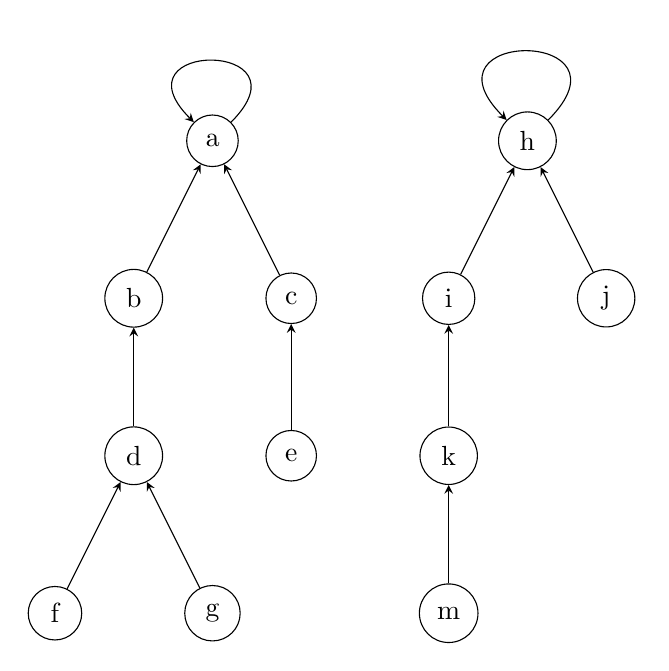
\begin{tikzpicture}[>=stealth]
    \node[ell] (a) at (3,6) {a};
    \node[ell] (b) at (2,4) {b};
    \node[ell] (c) at (4,4) {c};
    \node[ell] (d) at (2,2) {d};
    \node[ell] (e) at (4,2) {e};
    \node[ell] (f) at (1,0) {f};
    \node[ell] (g) at (3,0) {g};
    \node[ell] (h) at (7,6) {h};
    \node[ell] (i) at (6,4) {i};
    \node[ell] (j) at (8,4) {j};
    \node[ell] (k) at (6,2) {k};
    \node[ell] (m) at (6,0) {m};

    \draw [->] (a) to [loop]node[]{} (a);
    \draw [->] (b) to []node[]{} (a);
    \draw [->] (c) to []node[]{} (a);
    \draw [->] (d) to []node[]{} (b);
    \draw [->] (e) to []node[]{} (c);
    \draw [->] (f) to []node[]{} (d);
    \draw [->] (g) to []node[]{} (d);

    \draw [->] (h) to [loop]node[]{} (h);
    \draw [->] (i) to []node[]{} (h);
    \draw [->] (j) to []node[]{} (h);
    \draw [->] (k) to []node[]{} (i);
    \draw [->] (m) to []node[]{} (k);
\end{tikzpicture}
\caption{Disjoint-Set Forest}
\end{figure}
\\$UNION(f,m) \rightarrow LINK(FIND\_SET(f),FIND\_SET(m))$\\
\pagebreak
\\$FIND\_SET(f):$\hspace{2in}$FIND\_SET(m):$\\
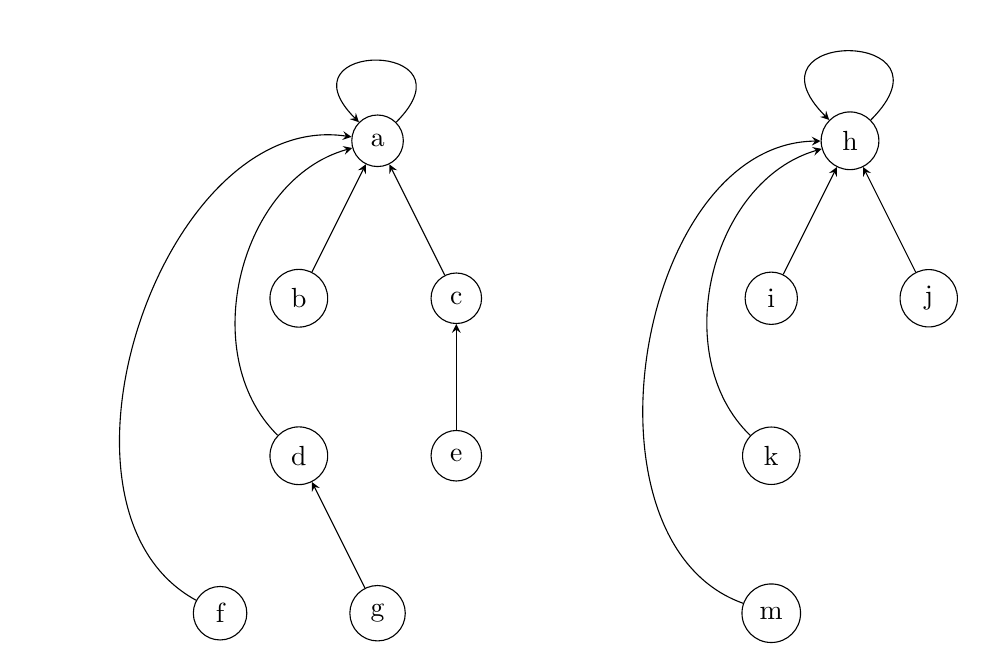
\begin{tikzpicture}[>=stealth]
    \node[ell] (a) at (3,6) {a};
    \node[ell] (b) at (2,4) {b};
    \node[ell] (c) at (4,4) {c};
    \node[ell] (d) at (2,2) {d};
    \node[ell] (e) at (4,2) {e};
    \node[ell] (f) at (1,0) {f};
    \node[ell] (g) at (3,0) {g};
    
    \node[ell] (h) at (9,6) {h};
    \node[ell] (i) at (8,4) {i};
    \node[ell] (j) at (10,4) {j};
    \node[ell] (k) at (8,2) {k};
    \node[ell] (m) at (8,0) {m};

    \draw [->] (a) to [loop]node[]{} (a);
    \draw [->] (b) to []node[]{} (a);
    \draw [->] (c) to []node[]{} (a);
    \draw [->] (d) to [bend left=60]node[]{} (a);
    \draw [->] (e) to []node[]{} (c);
    \draw [->] (f) to [bend left=80]node[]{} (a);
    \draw [->] (g) to []node[]{} (d);

    \draw [->] (h) to [loop]node[]{} (h);
    \draw [->] (i) to []node[]{} (h);
    \draw [->] (j) to []node[]{} (h);
    \draw [->] (k) to [bend left=60]node[]{} (h);
    \draw [->] (m) to [bend left=80]node[]{} (h);
\end{tikzpicture}
\\$LINK(FIND\_SET(f),FIND\_SET(m)):$\\
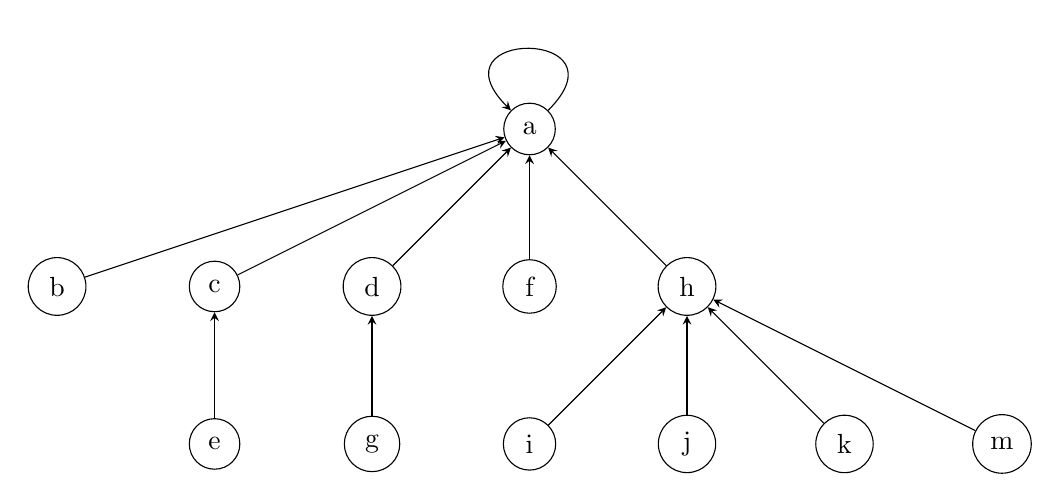
\begin{tikzpicture}[>=stealth]
    \node[ell] (a) at (6,6) {a};
    \node[ell] (b) at (0,4) {b};
    \node[ell] (c) at (2,4) {c};
    \node[ell] (d) at (4,4) {d};
    \node[ell] (e) at (2,2) {e};
    \node[ell] (f) at (6,4) {f};
    \node[ell] (g) at (4,2) {g};
    
    \node[ell] (h) at (8,4) {h};
    \node[ell] (i) at (6,2) {i};
    \node[ell] (j) at (8,2) {j};
    \node[ell] (k) at (10,2) {k};
    \node[ell] (m) at (12,2) {m};

    \draw [->] (a) to [loop]node[]{} (a);
    \draw [->] (b) to []node[]{} (a);
    \draw [->] (c) to []node[]{} (a);
    \draw [->] (d) to []node[]{} (a);
    \draw [->] (e) to []node[]{} (c);
    \draw [->] (f) to []node[]{} (a);
    \draw [->] (g) to []node[]{} (d);

    \draw [->] (h) to []node[]{} (a);
    \draw [->] (i) to []node[]{} (h);
    \draw [->] (j) to []node[]{} (h);
    \draw [->] (k) to []node[]{} (h);
    \draw [->] (m) to []node[]{} (h);
\end{tikzpicture}
\end{problem}
\pagebreak
\begin{problem}{2}
Extract the minimum node from the Fibonacci heap shown in figure 2.
\begin{figure}[h!]
    \centering
    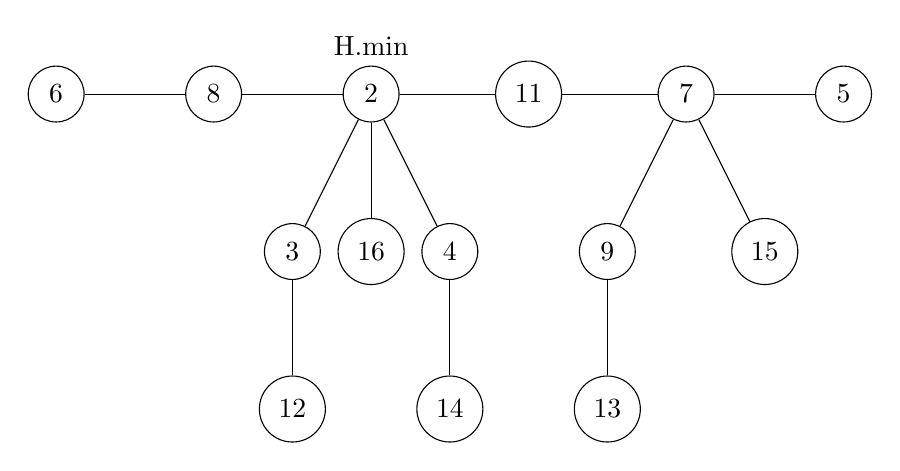
\begin{tikzpicture}[>=stealth]
        \node[ell] (a) at (0,6) {6};
        \node[ell] (b) at (2,6) {8};
        \node[ell,label={H.min}] (c) at (4,6) {2};
        \node[ell] (d) at (6,6) {11};
        \node[ell] (e) at (8,6) {7};
        \node[ell] (f) at (10,6) {5};
        \node[ell] (g) at (3,4) {3};
        \node[ell] (h) at (4,4) {16};
        \node[ell] (i) at (5,4) {4};
        \node[ell] (j) at (7,4) {9};
        \node[ell] (k) at (9,4) {15};
        \node[ell] (l) at (3,2) {12};
        \node[ell] (m) at (5,2) {14};
        \node[ell] (n) at (7,2) {13};

        \draw [] (a) to []node[]{} (b);
        \draw [] (b) to []node[]{} (c);
        \draw [] (c) to []node[]{} (d);
        \draw [] (d) to []node[]{} (e);
        \draw [] (e) to []node[]{} (f);
        \draw [] (g) to []node[]{} (c);
        \draw [] (h) to []node[]{} (c);
        \draw [] (i) to []node[]{} (c);
        \draw [] (j) to []node[]{} (e);
        \draw [] (k) to []node[]{} (e);
        \draw [] (l) to []node[]{} (g);
        \draw [] (m) to []node[]{} (i);
        \draw [] (n) to []node[]{} (j);
    \end{tikzpicture}
    \caption{Fibonacci Heap}
\end{figure}
\\After removing node 2 (previous H.min) and making roots out of each of its children:\\
\begin{tikzpicture}[>=stealth]
    \node[ell] (a) at (0,6) {6};
    \node[ell] (b) at (2,6) {8};
    \node[ell,label={H.min}] (d) at (10,6) {11};
    \node[ell] (e) at (12,6) {7};
    \node[ell] (f) at (14,6) {5};
    \node[ell] (g) at (4,6) {3};
    \node[ell] (h) at (6,6) {16};
    \node[ell] (i) at (8,6) {4};
    \node[ell] (j) at (11,4) {9};
    \node[ell] (k) at (13,4) {15};
    \node[ell] (l) at (4,4) {12};
    \node[ell] (m) at (8,4) {14};
    \node[ell] (n) at (11,2) {13};

    \draw [] (a) to []node[]{} (b);
    \draw [] (b) to []node[]{} (g);
    \draw [] (g) to []node[]{} (h);
    \draw [] (h) to []node[]{} (i);
    \draw [] (i) to []node[]{} (d);
    \draw [] (d) to []node[]{} (e);
    \draw [] (e) to []node[]{} (f);
    \draw [] (j) to []node[]{} (e);
    \draw [] (k) to []node[]{} (e);
    \draw [] (l) to []node[]{} (g);
    \draw [] (m) to []node[]{} (i);
    \draw [] (n) to []node[]{} (j);
\end{tikzpicture}
\\Since both node 11 and node 5 have degree 0, and $5 < 11$, link 11 to 5:\\
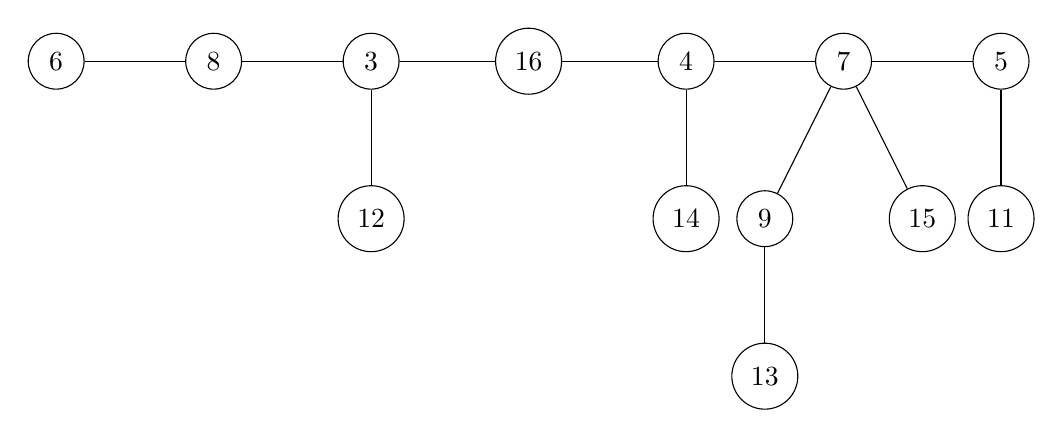
\begin{tikzpicture}[>=stealth]
    \node[ell] (a) at (0,6) {6};
    \node[ell] (b) at (2,6) {8};
    \node[ell] (d) at (12,4) {11};
    \node[ell] (e) at (10,6) {7};
    \node[ell] (f) at (12,6) {5};
    \node[ell] (g) at (4,6) {3};
    \node[ell] (h) at (6,6) {16};
    \node[ell] (i) at (8,6) {4};
    \node[ell] (j) at (9,4) {9};
    \node[ell] (k) at (11,4) {15};
    \node[ell] (l) at (4,4) {12};
    \node[ell] (m) at (8,4) {14};
    \node[ell] (n) at (9,2) {13};

    \draw [] (a) to []node[]{} (b);
    \draw [] (b) to []node[]{} (g);
    \draw [] (g) to []node[]{} (h);
    \draw [] (h) to []node[]{} (i);
    \draw [] (i) to []node[]{} (e);
    \draw [] (e) to []node[]{} (f);
    \draw [] (d) to []node[]{} (f);
    \draw [] (j) to []node[]{} (e);
    \draw [] (k) to []node[]{} (e);
    \draw [] (l) to []node[]{} (g);
    \draw [] (m) to []node[]{} (i);
    \draw [] (n) to []node[]{} (j);
\end{tikzpicture}
\pagebreak
\\Since both node 6 and node 8 have degree 0, and $6 < 8$, link 8 to 6:\\
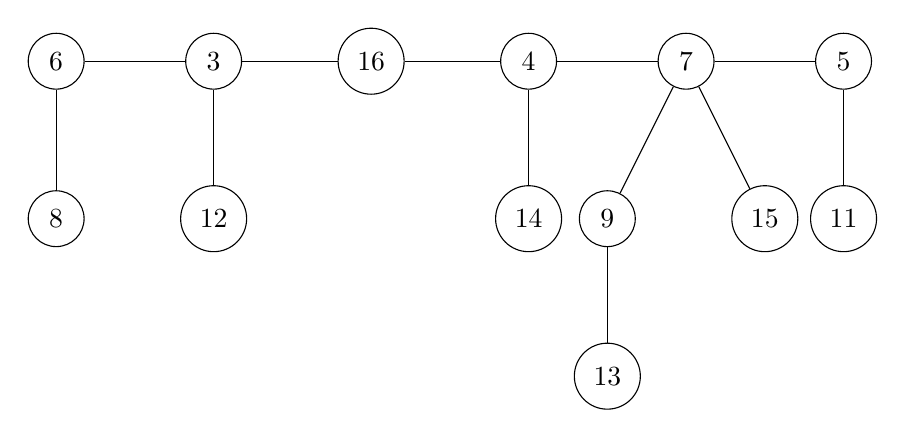
\begin{tikzpicture}[>=stealth]
    \node[ell] (b) at (2,4) {8};
    \node[ell] (a) at (2,6) {6};
    \node[ell] (d) at (12,4) {11};
    \node[ell] (e) at (10,6) {7};
    \node[ell] (f) at (12,6) {5};
    \node[ell] (g) at (4,6) {3};
    \node[ell] (h) at (6,6) {16};
    \node[ell] (i) at (8,6) {4};
    \node[ell] (j) at (9,4) {9};
    \node[ell] (k) at (11,4) {15};
    \node[ell] (l) at (4,4) {12};
    \node[ell] (m) at (8,4) {14};
    \node[ell] (n) at (9,2) {13};

    \draw [] (a) to []node[]{} (b);
    \draw [] (a) to []node[]{} (g);
    \draw [] (g) to []node[]{} (h);
    \draw [] (h) to []node[]{} (i);
    \draw [] (i) to []node[]{} (e);
    \draw [] (e) to []node[]{} (f);
    \draw [] (d) to []node[]{} (f);
    \draw [] (j) to []node[]{} (e);
    \draw [] (k) to []node[]{} (e);
    \draw [] (l) to []node[]{} (g);
    \draw [] (m) to []node[]{} (i);
    \draw [] (n) to []node[]{} (j);
\end{tikzpicture}
\\Since both node 6 and node 5 have degree 1, and $5 < 6$, link 6 to 5:\\
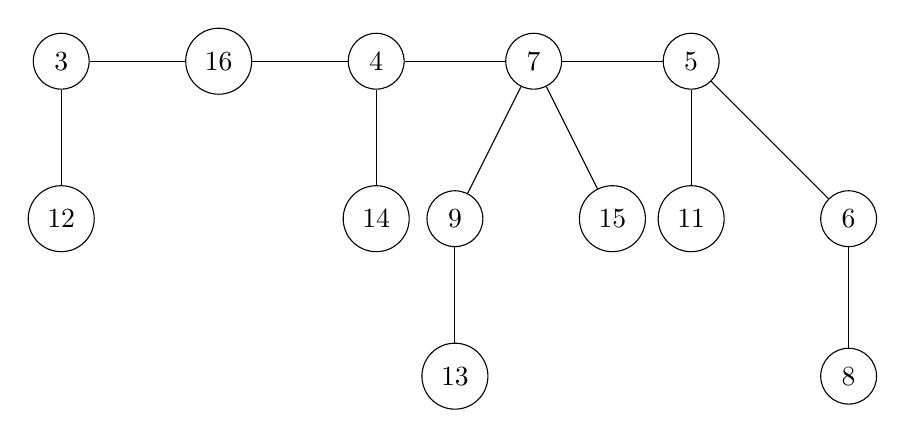
\begin{tikzpicture}[>=stealth]
    \node[ell] (b) at (14,2) {8};
    \node[ell] (a) at (14,4) {6};
    \node[ell] (d) at (12,4) {11};
    \node[ell] (e) at (10,6) {7};
    \node[ell] (f) at (12,6) {5};
    \node[ell] (g) at (4,6) {3};
    \node[ell] (h) at (6,6) {16};
    \node[ell] (i) at (8,6) {4};
    \node[ell] (j) at (9,4) {9};
    \node[ell] (k) at (11,4) {15};
    \node[ell] (l) at (4,4) {12};
    \node[ell] (m) at (8,4) {14};
    \node[ell] (n) at (9,2) {13};

    \draw [] (a) to []node[]{} (f);
    \draw [] (a) to []node[]{} (b);
    \draw [] (g) to []node[]{} (h);
    \draw [] (h) to []node[]{} (i);
    \draw [] (i) to []node[]{} (e);
    \draw [] (e) to []node[]{} (f);
    \draw [] (d) to []node[]{} (f);
    \draw [] (j) to []node[]{} (e);
    \draw [] (k) to []node[]{} (e);
    \draw [] (l) to []node[]{} (g);
    \draw [] (m) to []node[]{} (i);
    \draw [] (n) to []node[]{} (j);
\end{tikzpicture}
\\Since both node 7 and node 5 have degree 2, and $5 < 7$, link 7 to 5:\\
\begin{tikzpicture}[>=stealth]
    \node[ell] (b) at (14,2) {8};
    \node[ell] (a) at (14,4) {6};
    \node[ell] (d) at (12,4) {11};
    \node[ell] (e) at (10,4) {7};
    \node[ell] (f) at (12,6) {5};
    \node[ell] (g) at (4,6) {3};
    \node[ell] (h) at (6,6) {16};
    \node[ell] (i) at (8,6) {4};
    \node[ell] (j) at (9,2) {9};
    \node[ell] (k) at (11,2) {15};
    \node[ell] (l) at (4,4) {12};
    \node[ell] (m) at (8,4) {14};
    \node[ell] (n) at (9,0) {13};

    \draw [] (a) to []node[]{} (f);
    \draw [] (a) to []node[]{} (b);
    \draw [] (g) to []node[]{} (h);
    \draw [] (h) to []node[]{} (i);
    \draw [] (i) to []node[]{} (f);
    \draw [] (e) to []node[]{} (f);
    \draw [] (d) to []node[]{} (f);
    \draw [] (j) to []node[]{} (e);
    \draw [] (k) to []node[]{} (e);
    \draw [] (l) to []node[]{} (g);
    \draw [] (m) to []node[]{} (i);
    \draw [] (n) to []node[]{} (j);
\end{tikzpicture}
\pagebreak
\\Since both node 3 and node 4 have degree 1, and $3 < 4$, link 4 to 3, no more root nodes with same degree, so node 3 becomes new H.min:\\
\begin{tikzpicture}[>=stealth]
    \node[ell] (b) at (14,2) {8};
    \node[ell] (a) at (14,4) {6};
    \node[ell] (d) at (12,4) {11};
    \node[ell] (e) at (10,4) {7};
    \node[ell] (f) at (12,6) {5};
    \node[ell,label={H.min}] (g) at (4,6) {3};
    \node[ell] (h) at (6,6) {16};
    \node[ell] (i) at (6,4) {4};
    \node[ell] (j) at (9,2) {9};
    \node[ell] (k) at (11,2) {15};
    \node[ell] (l) at (4,4) {12};
    \node[ell] (m) at (6,2) {14};
    \node[ell] (n) at (9,0) {13};

    \draw [] (a) to []node[]{} (f);
    \draw [] (a) to []node[]{} (b);
    \draw [] (g) to []node[]{} (h);
    \draw [] (h) to []node[]{} (f);
    \draw [] (i) to []node[]{} (g);
    \draw [] (e) to []node[]{} (f);
    \draw [] (d) to []node[]{} (f);
    \draw [] (j) to []node[]{} (e);
    \draw [] (k) to []node[]{} (e);
    \draw [] (l) to []node[]{} (g);
    \draw [] (m) to []node[]{} (i);
    \draw [] (n) to []node[]{} (j);
\end{tikzpicture}
\end{problem}

\begin{problem}{3}
Perform Depth-First Search using Stack data structure on the (un)directed graph shown in figure
3. 
\begin{figure}[h!]
    \centering
    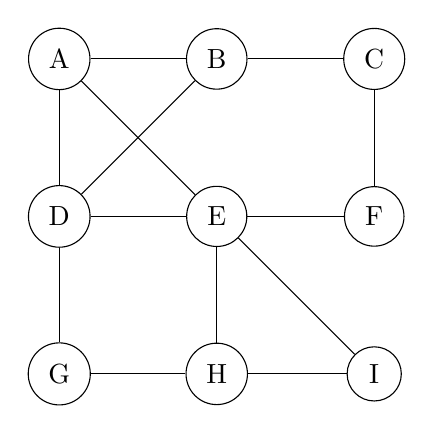
\begin{tikzpicture}[>=stealth]
        \node[ell] (a) at (0,6) {A};
        \node[ell] (b) at (2,6) {B};
        \node[ell] (c) at (4,6) {C};
        \node[ell] (d) at (0,4) {D};
        \node[ell] (e) at (2,4) {E};
        \node[ell] (f) at (4,4) {F};
        \node[ell] (g) at (0,2) {G};
        \node[ell] (h) at (2,2) {H};
        \node[ell] (i) at (4,2) {I};

        \draw [] (a) to []node[]{} (b);
        \draw [] (a) to []node[]{} (d);
        \draw [] (a) to []node[]{} (e);
        \draw [] (b) to []node[]{} (c);
        \draw [] (b) to []node[]{} (d);
        \draw [] (c) to []node[]{} (f);
        \draw [] (d) to []node[]{} (e);
        \draw [] (d) to []node[]{} (g);
        \draw [] (e) to []node[]{} (f);
        \draw [] (e) to []node[]{} (h);
        \draw [] (e) to []node[]{} (i);
        \draw [] (g) to []node[]{} (h);
        \draw [] (h) to []node[]{} (i);
    \end{tikzpicture}
    \caption{(Un)Directed Graph}
\end{figure}
\pagebreak
\\Randomly choose to start at H and go to E\\
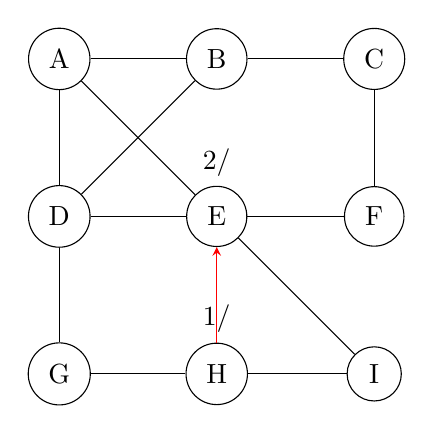
\begin{tikzpicture}[>=stealth]
    \node[ell] (a) at (0,6) {A};
    \node[ell] (b) at (2,6) {B};
    \node[ell] (c) at (4,6) {C};
    \node[ell] (d) at (0,4) {D};
    \node[ell,label={2/}] (e) at (2,4) {E};
    \node[ell] (f) at (4,4) {F};
    \node[ell] (g) at (0,2) {G};
    \node[ell,label={1/}] (h) at (2,2) {H};
    \node[ell] (i) at (4,2) {I};

    \draw [] (a) to []node[]{} (b);
    \draw [] (a) to []node[]{} (d);
    \draw [] (a) to []node[]{} (e);
    \draw [] (b) to []node[]{} (c);
    \draw [] (b) to []node[]{} (d);
    \draw [] (c) to []node[]{} (f);
    \draw [] (d) to []node[]{} (e);
    \draw [] (d) to []node[]{} (g);
    \draw [] (e) to []node[]{} (f);
    \draw [<-,red] (e) to []node[]{} (h);
    \draw [] (e) to []node[]{} (i);
    \draw [] (g) to []node[]{} (h);
    \draw [] (h) to []node[]{} (i);
\end{tikzpicture}
\begin{tabular}[b]{|c|} 
    \hline
    stack \\
    \hline
    \\
    \hline
    \\
    \hline
    \\
    \hline
    \\
    \hline
    \\
    \hline
    H\\
    \hline
\end{tabular}
$\rightarrow$
\begin{tabular}[b]{|c|} 
    \hline
    stack \\
    \hline
    \\
    \hline
    \\
    \hline
    \\
    \hline
    \\
    \hline
    E\\
    \hline
    H\\
    \hline
\end{tabular}
\\\\Randomly choose to go to I\\
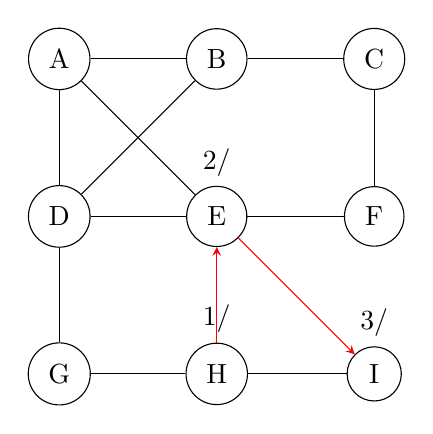
\begin{tikzpicture}[>=stealth]
    \node[ell] (a) at (0,6) {A};
    \node[ell] (b) at (2,6) {B};
    \node[ell] (c) at (4,6) {C};
    \node[ell] (d) at (0,4) {D};
    \node[ell,label={2/}] (e) at (2,4) {E};
    \node[ell] (f) at (4,4) {F};
    \node[ell] (g) at (0,2) {G};
    \node[ell,label={1/}] (h) at (2,2) {H};
    \node[ell,label={3/}] (i) at (4,2) {I};

    \draw [] (a) to []node[]{} (b);
    \draw [] (a) to []node[]{} (d);
    \draw [] (a) to []node[]{} (e);
    \draw [] (b) to []node[]{} (c);
    \draw [] (b) to []node[]{} (d);
    \draw [] (c) to []node[]{} (f);
    \draw [] (d) to []node[]{} (e);
    \draw [] (d) to []node[]{} (g);
    \draw [] (e) to []node[]{} (f);
    \draw [<-,red] (e) to []node[]{} (h);
    \draw [->,red] (e) to []node[]{} (i);
    \draw [] (g) to []node[]{} (h);
    \draw [] (h) to []node[]{} (i);
\end{tikzpicture}
\begin{tabular}[b]{|c|} 
    \hline
    stack \\
    \hline
    \\
    \hline
    \\
    \hline
    \\
    \hline
    \\
    \hline
    E\\
    \hline
    H\\
    \hline
\end{tabular}
$\rightarrow$
\begin{tabular}[b]{|c|} 
    \hline
    stack \\
    \hline
    \\
    \hline
    \\
    \hline
    \\
    \hline
    I\\
    \hline
    E\\
    \hline
    H\\
    \hline
\end{tabular}
\\\\I has no unvisited adjacent vertices, finish processing and pop from stack\\
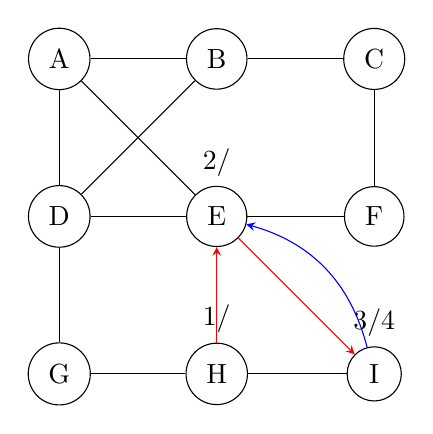
\begin{tikzpicture}[>=stealth]
    \node[ell] (a) at (0,6) {A};
    \node[ell] (b) at (2,6) {B};
    \node[ell] (c) at (4,6) {C};
    \node[ell] (d) at (0,4) {D};
    \node[ell,label={2/}] (e) at (2,4) {E};
    \node[ell] (f) at (4,4) {F};
    \node[ell] (g) at (0,2) {G};
    \node[ell,label={1/}] (h) at (2,2) {H};
    \node[ell,label={3/4}] (i) at (4,2) {I};

    \draw [] (a) to []node[]{} (b);
    \draw [] (a) to []node[]{} (d);
    \draw [] (a) to []node[]{} (e);
    \draw [] (b) to []node[]{} (c);
    \draw [] (b) to []node[]{} (d);
    \draw [] (c) to []node[]{} (f);
    \draw [] (d) to []node[]{} (e);
    \draw [] (d) to []node[]{} (g);
    \draw [] (e) to []node[]{} (f);
    \draw [<-,red] (e) to []node[]{} (h);
    \draw [->,red] (e) to []node[]{} (i);
    \draw [<-,blue] (e) to [bend left]node[]{} (i);
    \draw [] (g) to []node[]{} (h);
    \draw [] (h) to []node[]{} (i);
\end{tikzpicture}
\begin{tabular}[b]{|c|} 
    \hline
    stack \\
    \hline
    \\
    \hline
    \\
    \hline
    \\
    \hline
    I\\
    \hline
    E\\
    \hline
    H\\
    \hline
\end{tabular}
$\rightarrow$
\begin{tabular}[b]{|c|} 
    \hline
    stack \\
    \hline
    \\
    \hline
    \\
    \hline
    \\
    \hline
    \\
    \hline
    E\\
    \hline
    H\\
    \hline
\end{tabular}
\pagebreak
\\\\Randomly choose to go to D\\
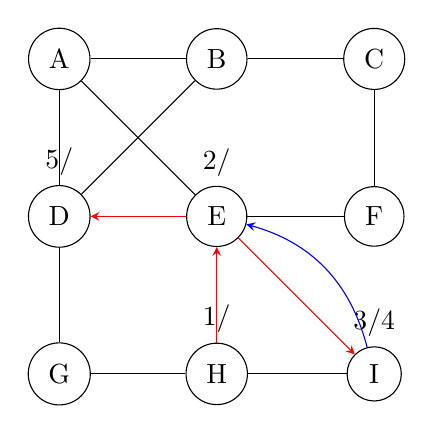
\begin{tikzpicture}[>=stealth]
    \node[ell] (a) at (0,6) {A};
    \node[ell] (b) at (2,6) {B};
    \node[ell] (c) at (4,6) {C};
    \node[ell,label={5/}] (d) at (0,4) {D};
    \node[ell,label={2/}] (e) at (2,4) {E};
    \node[ell] (f) at (4,4) {F};
    \node[ell] (g) at (0,2) {G};
    \node[ell,label={1/}] (h) at (2,2) {H};
    \node[ell,label={3/4}] (i) at (4,2) {I};

    \draw [] (a) to []node[]{} (b);
    \draw [] (a) to []node[]{} (d);
    \draw [] (a) to []node[]{} (e);
    \draw [] (b) to []node[]{} (c);
    \draw [] (b) to []node[]{} (d);
    \draw [] (c) to []node[]{} (f);
    \draw [<-,red] (d) to []node[]{} (e);
    \draw [] (d) to []node[]{} (g);
    \draw [] (e) to []node[]{} (f);
    \draw [<-,red] (e) to []node[]{} (h);
    \draw [->,red] (e) to []node[]{} (i);
    \draw [<-,blue] (e) to [bend left]node[]{} (i);
    \draw [] (g) to []node[]{} (h);
    \draw [] (h) to []node[]{} (i);
\end{tikzpicture}
\begin{tabular}[b]{|c|} 
    \hline
    stack \\
    \hline
    \\
    \hline
    \\
    \hline
    \\
    \hline
    \\
    \hline
    E\\
    \hline
    H\\
    \hline
\end{tabular}
$\rightarrow$
\begin{tabular}[b]{|c|} 
    \hline
    stack \\
    \hline
    \\
    \hline
    \\
    \hline
    \\
    \hline
    D\\
    \hline
    E\\
    \hline
    H\\
    \hline
\end{tabular}
\\\\Randomly choose to go to G\\
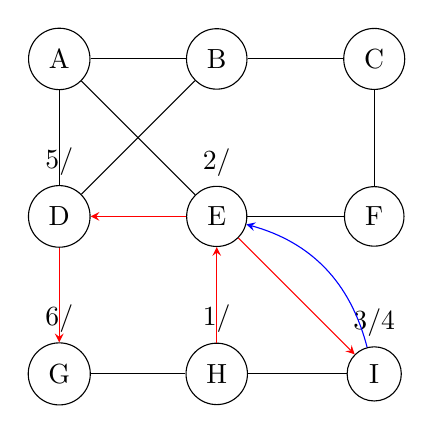
\begin{tikzpicture}[>=stealth]
    \node[ell] (a) at (0,6) {A};
    \node[ell] (b) at (2,6) {B};
    \node[ell] (c) at (4,6) {C};
    \node[ell,label={5/}] (d) at (0,4) {D};
    \node[ell,label={2/}] (e) at (2,4) {E};
    \node[ell] (f) at (4,4) {F};
    \node[ell,label={6/}] (g) at (0,2) {G};
    \node[ell,label={1/}] (h) at (2,2) {H};
    \node[ell,label={3/4}] (i) at (4,2) {I};

    \draw [] (a) to []node[]{} (b);
    \draw [] (a) to []node[]{} (d);
    \draw [] (a) to []node[]{} (e);
    \draw [] (b) to []node[]{} (c);
    \draw [] (b) to []node[]{} (d);
    \draw [] (c) to []node[]{} (f);
    \draw [<-,red] (d) to []node[]{} (e);
    \draw [->,red] (d) to []node[]{} (g);
    \draw [] (e) to []node[]{} (f);
    \draw [<-,red] (e) to []node[]{} (h);
    \draw [->,red] (e) to []node[]{} (i);
    \draw [<-,blue] (e) to [bend left]node[]{} (i);
    \draw [] (g) to []node[]{} (h);
    \draw [] (h) to []node[]{} (i);
\end{tikzpicture}
\begin{tabular}[b]{|c|} 
    \hline
    stack \\
    \hline
    \\
    \hline
    \\
    \hline
    \\
    \hline
    D\\
    \hline
    E\\
    \hline
    H\\
    \hline
\end{tabular}
$\rightarrow$
\begin{tabular}[b]{|c|} 
    \hline
    stack \\
    \hline
    \\
    \hline
    \\
    \hline
    G\\
    \hline
    D\\
    \hline
    E\\
    \hline
    H\\
    \hline
\end{tabular}
\\\\G has no unvisited adjacent vertices, finish processing and pop from stack\\
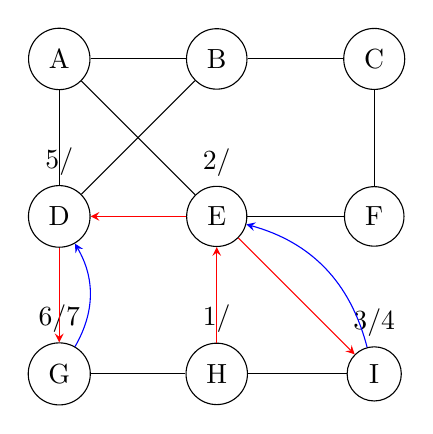
\begin{tikzpicture}[>=stealth]
    \node[ell] (a) at (0,6) {A};
    \node[ell] (b) at (2,6) {B};
    \node[ell] (c) at (4,6) {C};
    \node[ell,label={5/}] (d) at (0,4) {D};
    \node[ell,label={2/}] (e) at (2,4) {E};
    \node[ell] (f) at (4,4) {F};
    \node[ell,label={6/7}] (g) at (0,2) {G};
    \node[ell,label={1/}] (h) at (2,2) {H};
    \node[ell,label={3/4}] (i) at (4,2) {I};

    \draw [] (a) to []node[]{} (b);
    \draw [] (a) to []node[]{} (d);
    \draw [] (a) to []node[]{} (e);
    \draw [] (b) to []node[]{} (c);
    \draw [] (b) to []node[]{} (d);
    \draw [] (c) to []node[]{} (f);
    \draw [<-,red] (d) to []node[]{} (e);
    \draw [->,red] (d) to []node[]{} (g);
    \draw [<-,blue] (d) to [bend left]node[]{} (g);
    \draw [] (e) to []node[]{} (f);
    \draw [<-,red] (e) to []node[]{} (h);
    \draw [->,red] (e) to []node[]{} (i);
    \draw [<-,blue] (e) to [bend left]node[]{} (i);
    \draw [] (g) to []node[]{} (h);
    \draw [] (h) to []node[]{} (i);
\end{tikzpicture}
\begin{tabular}[b]{|c|} 
    \hline
    stack \\
    \hline
    \\
    \hline
    \\
    \hline
    G\\
    \hline
    D\\
    \hline
    E\\
    \hline
    H\\
    \hline
\end{tabular}
$\rightarrow$
\begin{tabular}[b]{|c|} 
    \hline
    stack \\
    \hline
    \\
    \hline
    \\
    \hline
    \\
    \hline
    D\\
    \hline
    E\\
    \hline
    H\\
    \hline
\end{tabular}
\pagebreak
\\\\Randomly choose to go to B\\
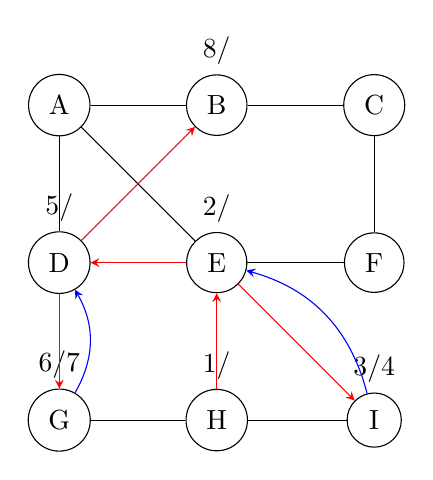
\begin{tikzpicture}[>=stealth]
    \node[ell] (a) at (0,6) {A};
    \node[ell,label={8/}] (b) at (2,6) {B};
    \node[ell] (c) at (4,6) {C};
    \node[ell,label={5/}] (d) at (0,4) {D};
    \node[ell,label={2/}] (e) at (2,4) {E};
    \node[ell] (f) at (4,4) {F};
    \node[ell,label={6/7}] (g) at (0,2) {G};
    \node[ell,label={1/}] (h) at (2,2) {H};
    \node[ell,label={3/4}] (i) at (4,2) {I};

    \draw [] (a) to []node[]{} (b);
    \draw [] (a) to []node[]{} (d);
    \draw [] (a) to []node[]{} (e);
    \draw [] (b) to []node[]{} (c);
    \draw [<-,red] (b) to []node[]{} (d);
    \draw [] (c) to []node[]{} (f);
    \draw [<-,red] (d) to []node[]{} (e);
    \draw [->,red] (d) to []node[]{} (g);
    \draw [<-,blue] (d) to [bend left]node[]{} (g);
    \draw [] (e) to []node[]{} (f);
    \draw [<-,red] (e) to []node[]{} (h);
    \draw [->,red] (e) to []node[]{} (i);
    \draw [<-,blue] (e) to [bend left]node[]{} (i);
    \draw [] (g) to []node[]{} (h);
    \draw [] (h) to []node[]{} (i);
\end{tikzpicture}
\begin{tabular}[b]{|c|} 
    \hline
    stack \\
    \hline
    \\
    \hline
    \\
    \hline
    \\
    \hline
    D\\
    \hline
    E\\
    \hline
    H\\
    \hline
\end{tabular}
$\rightarrow$
\begin{tabular}[b]{|c|} 
    \hline
    stack \\
    \hline
    \\
    \hline
    \\
    \hline
    B\\
    \hline
    D\\
    \hline
    E\\
    \hline
    H\\
    \hline
\end{tabular}
\\\\Randomly choose to go to C\\
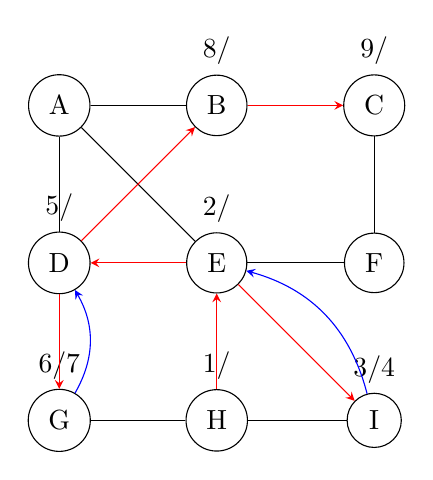
\begin{tikzpicture}[>=stealth]
    \node[ell] (a) at (0,6) {A};
    \node[ell,label={8/}] (b) at (2,6) {B};
    \node[ell,label={9/}] (c) at (4,6) {C};
    \node[ell,label={5/}] (d) at (0,4) {D};
    \node[ell,label={2/}] (e) at (2,4) {E};
    \node[ell] (f) at (4,4) {F};
    \node[ell,label={6/7}] (g) at (0,2) {G};
    \node[ell,label={1/}] (h) at (2,2) {H};
    \node[ell,label={3/4}] (i) at (4,2) {I};

    \draw [] (a) to []node[]{} (b);
    \draw [] (a) to []node[]{} (d);
    \draw [] (a) to []node[]{} (e);
    \draw [->,red] (b) to []node[]{} (c);
    \draw [<-,red] (b) to []node[]{} (d);
    \draw [] (c) to []node[]{} (f);
    \draw [<-,red] (d) to []node[]{} (e);
    \draw [->,red] (d) to []node[]{} (g);
    \draw [<-,blue] (d) to [bend left]node[]{} (g);
    \draw [] (e) to []node[]{} (f);
    \draw [<-,red] (e) to []node[]{} (h);
    \draw [->,red] (e) to []node[]{} (i);
    \draw [<-,blue] (e) to [bend left]node[]{} (i);
    \draw [] (g) to []node[]{} (h);
    \draw [] (h) to []node[]{} (i);
\end{tikzpicture}
\begin{tabular}[b]{|c|} 
    \hline
    stack \\
    \hline
    \\
    \hline
    \\
    \hline
    B\\
    \hline
    D\\
    \hline
    E\\
    \hline
    H\\
    \hline
\end{tabular}
$\rightarrow$
\begin{tabular}[b]{|c|} 
    \hline
    stack \\
    \hline
    \\
    \hline
    C\\
    \hline
    B\\
    \hline
    D\\
    \hline
    E\\
    \hline
    H\\
    \hline
\end{tabular}
\\\\Randomly choose to go to F\\
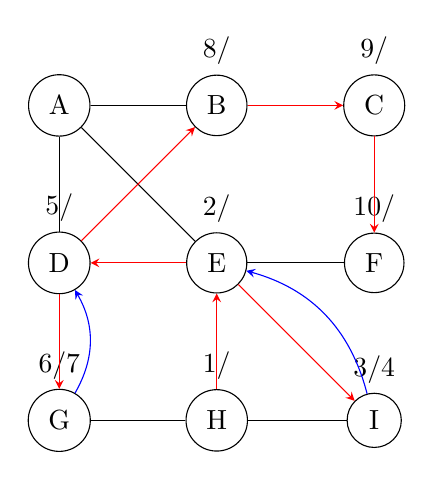
\begin{tikzpicture}[>=stealth]
    \node[ell] (a) at (0,6) {A};
    \node[ell,label={8/}] (b) at (2,6) {B};
    \node[ell,label={9/}] (c) at (4,6) {C};
    \node[ell,label={5/}] (d) at (0,4) {D};
    \node[ell,label={2/}] (e) at (2,4) {E};
    \node[ell,label={10/}] (f) at (4,4) {F};
    \node[ell,label={6/7}] (g) at (0,2) {G};
    \node[ell,label={1/}] (h) at (2,2) {H};
    \node[ell,label={3/4}] (i) at (4,2) {I};

    \draw [] (a) to []node[]{} (b);
    \draw [] (a) to []node[]{} (d);
    \draw [] (a) to []node[]{} (e);
    \draw [->,red] (b) to []node[]{} (c);
    \draw [<-,red] (b) to []node[]{} (d);
    \draw [->,red] (c) to []node[]{} (f);
    \draw [<-,red] (d) to []node[]{} (e);
    \draw [->,red] (d) to []node[]{} (g);
    \draw [<-,blue] (d) to [bend left]node[]{} (g);
    \draw [] (e) to []node[]{} (f);
    \draw [<-,red] (e) to []node[]{} (h);
    \draw [->,red] (e) to []node[]{} (i);
    \draw [<-,blue] (e) to [bend left]node[]{} (i);
    \draw [] (g) to []node[]{} (h);
    \draw [] (h) to []node[]{} (i);
\end{tikzpicture}
\begin{tabular}[b]{|c|} 
    \hline
    stack \\
    \hline
    \\
    \hline
    C\\
    \hline
    B\\
    \hline
    D\\
    \hline
    E\\
    \hline
    H\\
    \hline
\end{tabular}
$\rightarrow$
\begin{tabular}[b]{|c|} 
    \hline
    stack \\
    \hline
    F\\
    \hline
    C\\
    \hline
    B\\
    \hline
    D\\
    \hline
    E\\
    \hline
    H\\
    \hline
\end{tabular}
\pagebreak
\\\\F has no unvisited adjacent vertices, finish processing and pop from stack\\
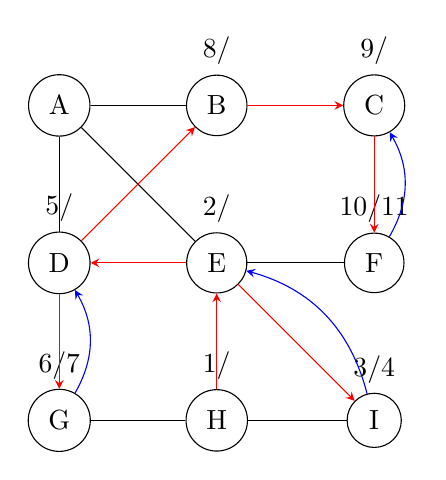
\begin{tikzpicture}[>=stealth]
    \node[ell] (a) at (0,6) {A};
    \node[ell,label={8/}] (b) at (2,6) {B};
    \node[ell,label={9/}] (c) at (4,6) {C};
    \node[ell,label={5/}] (d) at (0,4) {D};
    \node[ell,label={2/}] (e) at (2,4) {E};
    \node[ell,label={10/11}] (f) at (4,4) {F};
    \node[ell,label={6/7}] (g) at (0,2) {G};
    \node[ell,label={1/}] (h) at (2,2) {H};
    \node[ell,label={3/4}] (i) at (4,2) {I};

    \draw [] (a) to []node[]{} (b);
    \draw [] (a) to []node[]{} (d);
    \draw [] (a) to []node[]{} (e);
    \draw [->,red] (b) to []node[]{} (c);
    \draw [<-,red] (b) to []node[]{} (d);
    \draw [->,red] (c) to []node[]{} (f);
    \draw [<-,blue] (c) to [bend left]node[]{} (f);
    \draw [<-,red] (d) to []node[]{} (e);
    \draw [->,red] (d) to []node[]{} (g);
    \draw [<-,blue] (d) to [bend left]node[]{} (g);
    \draw [] (e) to []node[]{} (f);
    \draw [<-,red] (e) to []node[]{} (h);
    \draw [->,red] (e) to []node[]{} (i);
    \draw [<-,blue] (e) to [bend left]node[]{} (i);
    \draw [] (g) to []node[]{} (h);
    \draw [] (h) to []node[]{} (i);
\end{tikzpicture}
\begin{tabular}[b]{|c|} 
    \hline
    stack \\
    \hline
    F\\
    \hline
    C\\
    \hline
    B\\
    \hline
    D\\
    \hline
    E\\
    \hline
    H\\
    \hline
\end{tabular}
$\rightarrow$
\begin{tabular}[b]{|c|} 
    \hline
    stack \\
    \hline
    \\
    \hline
    C\\
    \hline
    B\\
    \hline
    D\\
    \hline
    E\\
    \hline
    H\\
    \hline
\end{tabular}
\\\\C has no unvisited adjacent vertices, finish processing and pop from stack\\
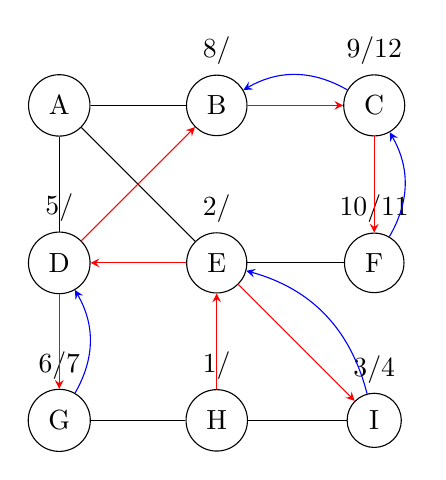
\begin{tikzpicture}[>=stealth]
    \node[ell] (a) at (0,6) {A};
    \node[ell,label={8/}] (b) at (2,6) {B};
    \node[ell,label={9/12}] (c) at (4,6) {C};
    \node[ell,label={5/}] (d) at (0,4) {D};
    \node[ell,label={2/}] (e) at (2,4) {E};
    \node[ell,label={10/11}] (f) at (4,4) {F};
    \node[ell,label={6/7}] (g) at (0,2) {G};
    \node[ell,label={1/}] (h) at (2,2) {H};
    \node[ell,label={3/4}] (i) at (4,2) {I};

    \draw [] (a) to []node[]{} (b);
    \draw [] (a) to []node[]{} (d);
    \draw [] (a) to []node[]{} (e);
    \draw [->,red] (b) to []node[]{} (c);
    \draw [<-,blue] (b) to [bend left]node[]{} (c);
    \draw [<-,red] (b) to []node[]{} (d);
    \draw [->,red] (c) to []node[]{} (f);
    \draw [<-,blue] (c) to [bend left]node[]{} (f);
    \draw [<-,red] (d) to []node[]{} (e);
    \draw [->,red] (d) to []node[]{} (g);
    \draw [<-,blue] (d) to [bend left]node[]{} (g);
    \draw [] (e) to []node[]{} (f);
    \draw [<-,red] (e) to []node[]{} (h);
    \draw [->,red] (e) to []node[]{} (i);
    \draw [<-,blue] (e) to [bend left]node[]{} (i);
    \draw [] (g) to []node[]{} (h);
    \draw [] (h) to []node[]{} (i);
\end{tikzpicture}
\begin{tabular}[b]{|c|} 
    \hline
    stack \\
    \hline
    \\
    \hline
    C\\
    \hline
    B\\
    \hline
    D\\
    \hline
    E\\
    \hline
    H\\
    \hline
\end{tabular}
$\rightarrow$
\begin{tabular}[b]{|c|} 
    \hline
    stack \\
    \hline
    \\
    \hline
    \\
    \hline
    B\\
    \hline
    D\\
    \hline
    E\\
    \hline
    H\\
    \hline
\end{tabular}
\\\\Randomly choose to go to A\\
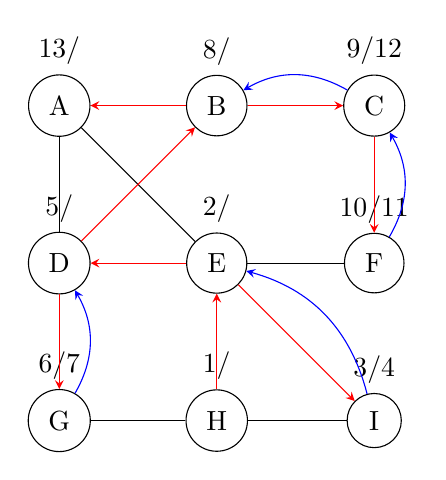
\begin{tikzpicture}[>=stealth]
    \node[ell,label={13/}] (a) at (0,6) {A};
    \node[ell,label={8/}] (b) at (2,6) {B};
    \node[ell,label={9/12}] (c) at (4,6) {C};
    \node[ell,label={5/}] (d) at (0,4) {D};
    \node[ell,label={2/}] (e) at (2,4) {E};
    \node[ell,label={10/11}] (f) at (4,4) {F};
    \node[ell,label={6/7}] (g) at (0,2) {G};
    \node[ell,label={1/}] (h) at (2,2) {H};
    \node[ell,label={3/4}] (i) at (4,2) {I};

    \draw [<-,red] (a) to []node[]{} (b);
    \draw [] (a) to []node[]{} (d);
    \draw [] (a) to []node[]{} (e);
    \draw [->,red] (b) to []node[]{} (c);
    \draw [<-,blue] (b) to [bend left]node[]{} (c);
    \draw [<-,red] (b) to []node[]{} (d);
    \draw [->,red] (c) to []node[]{} (f);
    \draw [<-,blue] (c) to [bend left]node[]{} (f);
    \draw [<-,red] (d) to []node[]{} (e);
    \draw [->,red] (d) to []node[]{} (g);
    \draw [<-,blue] (d) to [bend left]node[]{} (g);
    \draw [] (e) to []node[]{} (f);
    \draw [<-,red] (e) to []node[]{} (h);
    \draw [->,red] (e) to []node[]{} (i);
    \draw [<-,blue] (e) to [bend left]node[]{} (i);
    \draw [] (g) to []node[]{} (h);
    \draw [] (h) to []node[]{} (i);
\end{tikzpicture}
\begin{tabular}[b]{|c|} 
    \hline
    stack \\
    \hline
    \\
    \hline
    \\
    \hline
    B\\
    \hline
    D\\
    \hline
    E\\
    \hline
    H\\
    \hline
\end{tabular}
$\rightarrow$
\begin{tabular}[b]{|c|} 
    \hline
    stack \\
    \hline
    \\
    \hline
    A\\
    \hline
    B\\
    \hline
    D\\
    \hline
    E\\
    \hline
    H\\
    \hline
\end{tabular}
\pagebreak
\\\\All nodes visited, finish processing and pop until stack empy\\
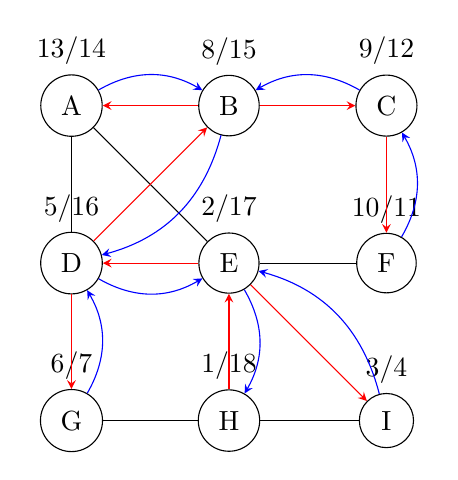
\begin{tikzpicture}[>=stealth]
    \node[ell,label={13/14}] (a) at (0,6) {A};
    \node[ell,label={8/15}] (b) at (2,6) {B};
    \node[ell,label={9/12}] (c) at (4,6) {C};
    \node[ell,label={5/16}] (d) at (0,4) {D};
    \node[ell,label={2/17}] (e) at (2,4) {E};
    \node[ell,label={10/11}] (f) at (4,4) {F};
    \node[ell,label={6/7}] (g) at (0,2) {G};
    \node[ell,label={1/18}] (h) at (2,2) {H};
    \node[ell,label={3/4}] (i) at (4,2) {I};

    \draw [<-,red] (a) to []node[]{} (b);
    \draw [->,blue] (a) to [bend left]node[]{} (b);
    \draw [] (a) to []node[]{} (d);
    \draw [] (a) to []node[]{} (e);
    \draw [->,red] (b) to []node[]{} (c);
    \draw [<-,blue] (b) to [bend left]node[]{} (c);
    \draw [<-,red] (b) to []node[]{} (d);
    \draw [->,blue] (b) to [bend left]node[]{} (d);
    \draw [->,red] (c) to []node[]{} (f);
    \draw [<-,blue] (c) to [bend left]node[]{} (f);
    \draw [<-,red] (d) to []node[]{} (e);
    \draw [->,blue] (d) to [bend right]node[]{} (e);
    \draw [->,red] (d) to []node[]{} (g);
    \draw [<-,blue] (d) to [bend left]node[]{} (g);
    \draw [] (e) to []node[]{} (f);
    \draw [<-,red] (e) to []node[]{} (h);
    \draw [->,blue] (e) to [bend left]node[]{} (h);
    \draw [->,red] (e) to []node[]{} (i);
    \draw [<-,blue] (e) to [bend left]node[]{} (i);
    \draw [] (g) to []node[]{} (h);
    \draw [] (h) to []node[]{} (i);
\end{tikzpicture}
\begin{tabular}[b]{|c|} 
    \hline
    stack \\
    \hline
    \\
    \hline
    A\\
    \hline
    B\\
    \hline
    D\\
    \hline
    E\\
    \hline
    H\\
    \hline
\end{tabular}
$\rightarrow$
\begin{tabular}[b]{|c|} 
    \hline
    stack \\
    \hline
    \\
    \hline
    \\
    \hline
    B\\
    \hline
    D\\
    \hline
    E\\
    \hline
    H\\
    \hline
\end{tabular}
$\rightarrow$
\begin{tabular}[b]{|c|} 
    \hline
    stack \\
    \hline
    \\
    \hline
    \\
    \hline
    \\
    \hline
    D\\
    \hline
    E\\
    \hline
    H\\
    \hline
\end{tabular}
$\rightarrow$
\begin{tabular}[b]{|c|} 
    \hline
    stack \\
    \hline
    \\
    \hline
    \\
    \hline
    \\
    \hline
    \\
    \hline
    E\\
    \hline
    H\\
    \hline
\end{tabular}
$\rightarrow$
\begin{tabular}[b]{|c|} 
    \hline
    stack \\
    \hline
    \\
    \hline
    \\
    \hline
    \\
    \hline
    \\
    \hline
    \\
    \hline
    H\\
    \hline
\end{tabular}
$\rightarrow$
\begin{tabular}[b]{|c|} 
    \hline
    stack \\
    \hline
    \\
    \hline
    \\
    \hline
    \\
    \hline
    \\
    \hline
    \\
    \hline
    \\
    \hline
\end{tabular}
\end{problem}
\pagebreak
\begin{problem}{4}
Using Prim's algorithm find the minimum spanning tree for the graph shown in figure 4\\
\begin{figure}[h!]
    \centering
    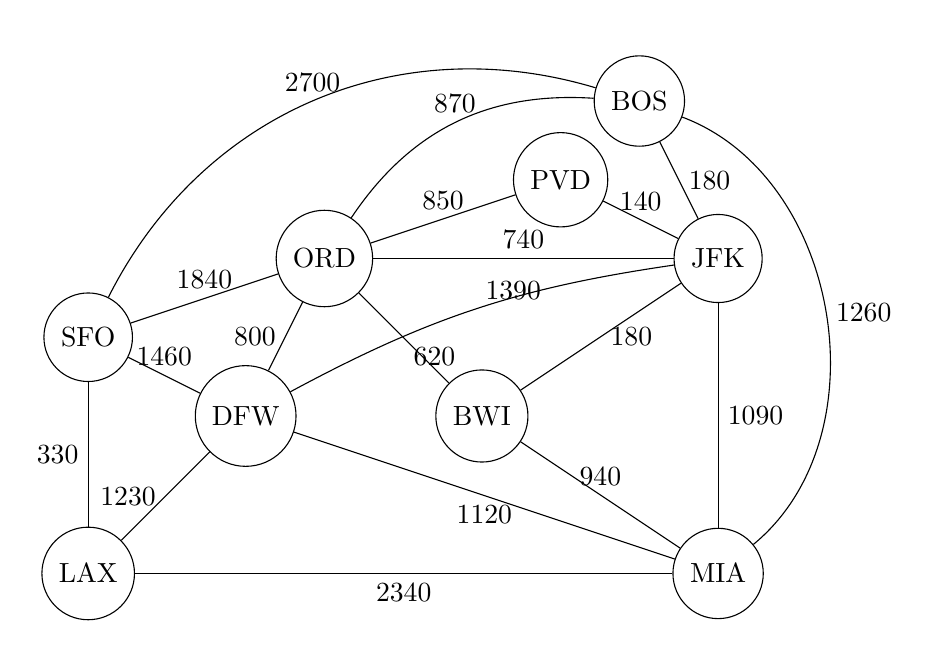
\begin{tikzpicture}[>=stealth]
        \node[ell] (sfo) at (1,8) {SFO};
        \node[ell] (lax) at (1,5) {LAX};
        \node[ell] (dfw) at (3,7) {DFW};
        \node[ell] (ord) at (4,9) {ORD};
        \node[ell] (bos) at (8,11) {BOS};
        \node[ell] (pvd) at (7,10) {PVD};
        \node[ell] (jfk) at (9,9) {JFK};
        \node[ell] (bwi) at (6,7) {BWI};
        \node[ell] (mia) at (9,5) {MIA};

        \draw [] (sfo) to []node[left]{330} (lax);
        \draw [] (sfo) to [bend left=40]node[above]{2700} (bos);
        \draw [] (sfo) to []node[above]{1840} (ord);
        \draw [] (sfo) to []node[above]{1460} (dfw);
        \draw [] (lax) to []node[left]{1230} (dfw);
        \draw [] (lax) to []node[below]{2340} (mia);
        \draw [] (dfw) to []node[left]{800} (ord);
        \draw [] (dfw) to [bend left=10]node[above right]{1390} (jfk);
        \draw [] (dfw) to []node[below]{1120} (mia);
        \draw [] (ord) to []node[below right]{620} (bwi);
        \draw [] (ord) to []node[above]{740} (jfk);
        \draw [] (ord) to []node[above]{850} (pvd);
        \draw [] (ord) to [bend left]node[above]{870} (bos);
        \draw [] (pvd) to []node[above]{140} (jfk);
        \draw [] (bos) to []node[right]{180} (jfk);
        \draw [] (bos) to [bend left=60]node[right]{1260} (mia);
        \draw [] (jfk) to []node[right]{180} (bwi);
        \draw [] (jfk) to []node[right]{1090} (mia);
        \draw [] (mia) to []node[above]{940} (bwi);

    \end{tikzpicture}
    \caption{Undirected Graph for Problem 4 and 5}
\end{figure}
\\Start at SFO, add 330 to LAX. From LAX, add 1230 to DFW.
\\From DFW, add 800 to ORD. From ORD, add 620 to BWI.
\\From BWI, add 180 to JFK. From JFK, add 140 to PVD.
\\From JFK, add 180 to BOS. From BWI, add 940 to MIA.\\
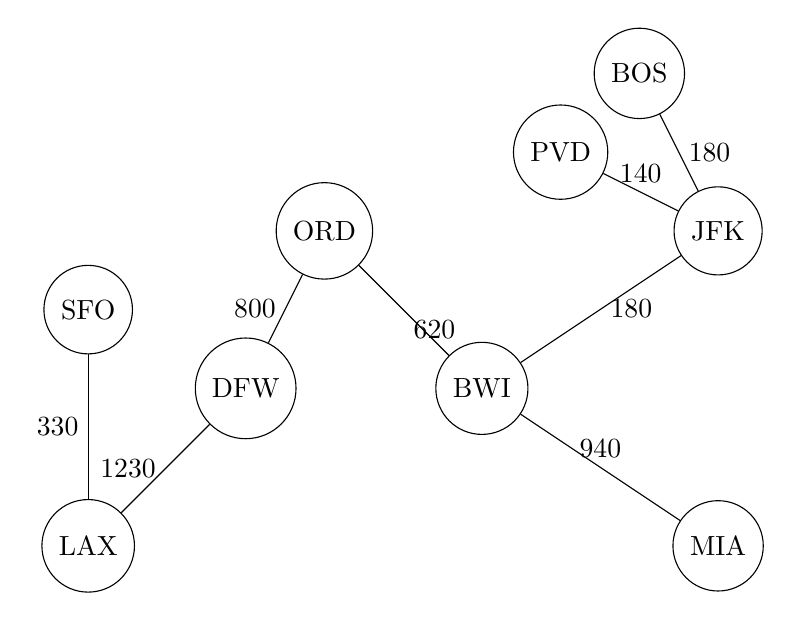
\begin{tikzpicture}[>=stealth]
    \node[ell] (sfo) at (1,8) {SFO};
    \node[ell] (lax) at (1,5) {LAX};
    \node[ell] (dfw) at (3,7) {DFW};
    \node[ell] (ord) at (4,9) {ORD};
    \node[ell] (bos) at (8,11) {BOS};
    \node[ell] (pvd) at (7,10) {PVD};
    \node[ell] (jfk) at (9,9) {JFK};
    \node[ell] (bwi) at (6,7) {BWI};
    \node[ell] (mia) at (9,5) {MIA};

    \draw [] (sfo) to []node[left]{330} (lax);
    \draw [] (lax) to []node[left]{1230} (dfw);
    \draw [] (dfw) to []node[left]{800} (ord);
    \draw [] (ord) to []node[below right]{620} (bwi);
    \draw [] (bwi) to []node[right]{180} (jfk);
    \draw [] (jfk) to []node[above]{140} (pvd);
    \draw [] (bos) to []node[right]{180} (jfk);
    \draw [] (bwi) to []node[above]{940} (mia);
\end{tikzpicture}
\end{problem}
\pagebreak
\begin{problem}{5}
    Using Dijkstra's algorithm find the shortest paths from the source vertex DFW to all the other
    vertices for the graph shown in figure 4. Note that Dijkstra's algorithm can be applied both on
    directed and undirected graph.

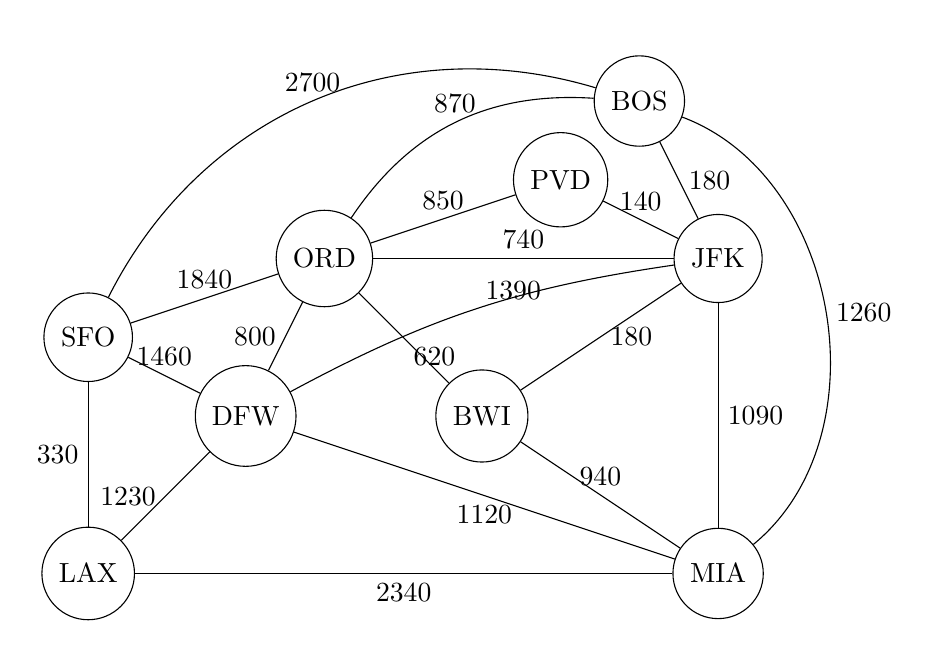
\begin{tikzpicture}[>=stealth]
    \node[ell] (sfo) at (1,8) {SFO};
    \node[ell] (lax) at (1,5) {LAX};
    \node[ell] (dfw) at (3,7) {DFW};
    \node[ell] (ord) at (4,9) {ORD};
    \node[ell] (bos) at (8,11) {BOS};
    \node[ell] (pvd) at (7,10) {PVD};
    \node[ell] (jfk) at (9,9) {JFK};
    \node[ell] (bwi) at (6,7) {BWI};
    \node[ell] (mia) at (9,5) {MIA};

    \draw [] (sfo) to []node[left]{330} (lax);
    \draw [] (sfo) to [bend left=40]node[above]{2700} (bos);
    \draw [] (sfo) to []node[above]{1840} (ord);
    \draw [] (sfo) to []node[above]{1460} (dfw);
    \draw [] (lax) to []node[left]{1230} (dfw);
    \draw [] (lax) to []node[below]{2340} (mia);
    \draw [] (dfw) to []node[left]{800} (ord);
    \draw [] (dfw) to [bend left=10]node[above right]{1390} (jfk);
    \draw [] (dfw) to []node[below]{1120} (mia);
    \draw [] (ord) to []node[below right]{620} (bwi);
    \draw [] (ord) to []node[above]{740} (jfk);
    \draw [] (ord) to []node[above]{850} (pvd);
    \draw [] (ord) to [bend left]node[above]{870} (bos);
    \draw [] (pvd) to []node[above]{140} (jfk);
    \draw [] (bos) to []node[right]{180} (jfk);
    \draw [] (bos) to [bend left=60]node[right]{1260} (mia);
    \draw [] (jfk) to []node[right]{180} (bwi);
    \draw [] (jfk) to []node[right]{1090} (mia);
    \draw [] (mia) to []node[above]{940} (bwi);
\end{tikzpicture}
\begin{tabular}[b]{|c c c|} 
    \hline
    vertex $v$ & $v.d$ & $v.\pi$ \\
    \hline
    DFW & 0 & nil\\
    SFO & $\infty$ & nil \\
    LAX & $\infty$ & nil \\
    ORD & $\infty$ & nil \\
    BOS & $\infty$ & nil \\
    PVD & $\infty$ & nil \\
    JFK & $\infty$ & nil \\
    BWI & $\infty$ & nil \\
    MIA & $\infty$ & nil \\
    \hline
\end{tabular}
\\
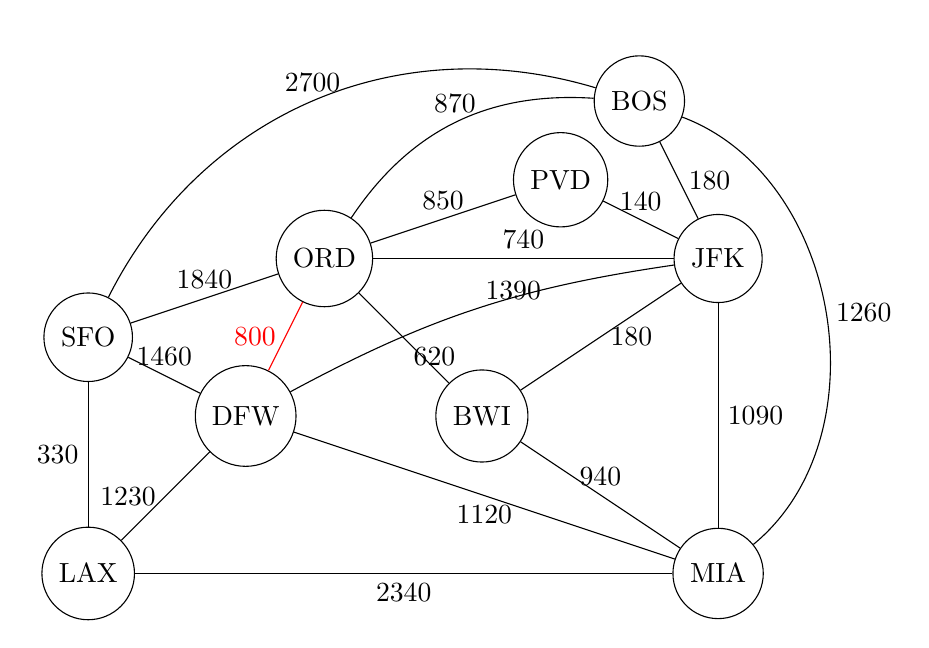
\begin{tikzpicture}[>=stealth]
    \node[ell] (sfo) at (1,8) {SFO};
    \node[ell] (lax) at (1,5) {LAX};
    \node[ell] (dfw) at (3,7) {DFW};
    \node[ell] (ord) at (4,9) {ORD};
    \node[ell] (bos) at (8,11) {BOS};
    \node[ell] (pvd) at (7,10) {PVD};
    \node[ell] (jfk) at (9,9) {JFK};
    \node[ell] (bwi) at (6,7) {BWI};
    \node[ell] (mia) at (9,5) {MIA};

    \draw [] (sfo) to []node[left]{330} (lax);
    \draw [] (sfo) to [bend left=40]node[above]{2700} (bos);
    \draw [] (sfo) to []node[above]{1840} (ord);
    \draw [] (sfo) to []node[above]{1460} (dfw);
    \draw [] (lax) to []node[left]{1230} (dfw);
    \draw [] (lax) to []node[below]{2340} (mia);
    \draw [red] (dfw) to []node[left]{800} (ord);
    \draw [] (dfw) to [bend left=10]node[above right]{1390} (jfk);
    \draw [] (dfw) to []node[below]{1120} (mia);
    \draw [] (ord) to []node[below right]{620} (bwi);
    \draw [] (ord) to []node[above]{740} (jfk);
    \draw [] (ord) to []node[above]{850} (pvd);
    \draw [] (ord) to [bend left]node[above]{870} (bos);
    \draw [] (pvd) to []node[above]{140} (jfk);
    \draw [] (bos) to []node[right]{180} (jfk);
    \draw [] (bos) to [bend left=60]node[right]{1260} (mia);
    \draw [] (jfk) to []node[right]{180} (bwi);
    \draw [] (jfk) to []node[right]{1090} (mia);
    \draw [] (mia) to []node[above]{940} (bwi);
\end{tikzpicture}
\begin{tabular}[b]{|c c c|} 
    \hline
    vertex $v$ & $v.d$ & $v.\pi$ \\
    \hline
    DFW & 0 & nil\\
    SFO & $\infty$ & nil \\
    LAX & $\infty$ & nil \\
    ORD & $800$ & DFW \\
    BOS & $\infty$ & nil \\
    PVD & $\infty$ & nil \\
    JFK & $\infty$ & nil \\
    BWI & $\infty$ & nil \\
    MIA & $\infty$ & nil \\
    \hline
\end{tabular}
\\
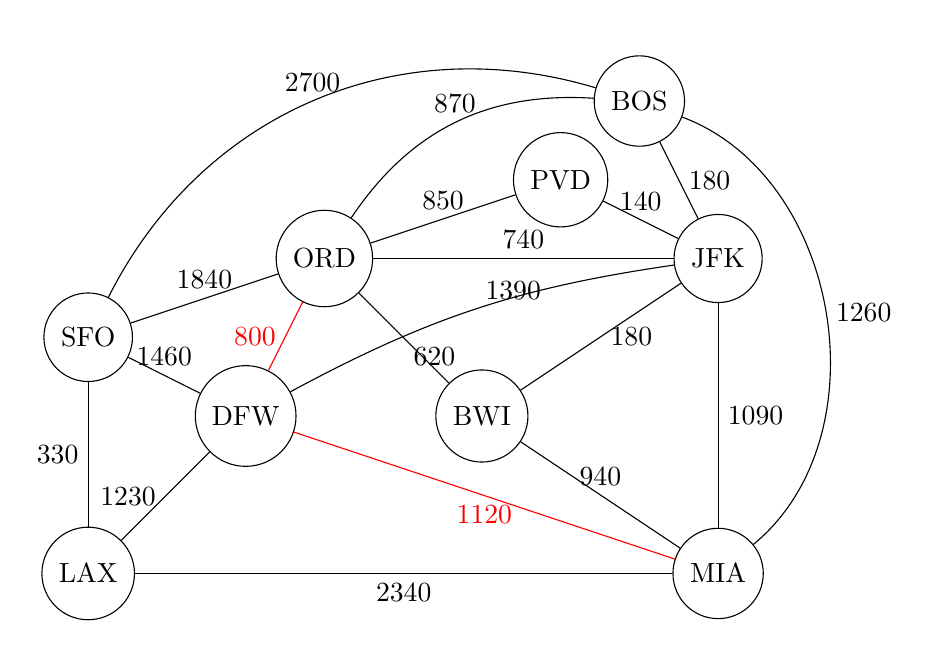
\begin{tikzpicture}[>=stealth]
    \node[ell] (sfo) at (1,8) {SFO};
    \node[ell] (lax) at (1,5) {LAX};
    \node[ell] (dfw) at (3,7) {DFW};
    \node[ell] (ord) at (4,9) {ORD};
    \node[ell] (bos) at (8,11) {BOS};
    \node[ell] (pvd) at (7,10) {PVD};
    \node[ell] (jfk) at (9,9) {JFK};
    \node[ell] (bwi) at (6,7) {BWI};
    \node[ell] (mia) at (9,5) {MIA};

    \draw [] (sfo) to []node[left]{330} (lax);
    \draw [] (sfo) to [bend left=40]node[above]{2700} (bos);
    \draw [] (sfo) to []node[above]{1840} (ord);
    \draw [] (sfo) to []node[above]{1460} (dfw);
    \draw [] (lax) to []node[left]{1230} (dfw);
    \draw [] (lax) to []node[below]{2340} (mia);
    \draw [red] (dfw) to []node[left]{800} (ord);
    \draw [] (dfw) to [bend left=10]node[above right]{1390} (jfk);
    \draw [red] (dfw) to []node[below]{1120} (mia);
    \draw [] (ord) to []node[below right]{620} (bwi);
    \draw [] (ord) to []node[above]{740} (jfk);
    \draw [] (ord) to []node[above]{850} (pvd);
    \draw [] (ord) to [bend left]node[above]{870} (bos);
    \draw [] (pvd) to []node[above]{140} (jfk);
    \draw [] (bos) to []node[right]{180} (jfk);
    \draw [] (bos) to [bend left=60]node[right]{1260} (mia);
    \draw [] (jfk) to []node[right]{180} (bwi);
    \draw [] (jfk) to []node[right]{1090} (mia);
    \draw [] (mia) to []node[above]{940} (bwi);
\end{tikzpicture}
\begin{tabular}[b]{|c c c|} 
    \hline
    vertex $v$ & $v.d$ & $v.\pi$ \\
    \hline
    DFW & 0 & nil\\
    SFO & $\infty$ & nil \\
    LAX & $\infty$ & nil \\
    ORD & 800 & DFW \\
    BOS & $\infty$ & nil \\
    PVD & $\infty$ & nil \\
    JFK & $\infty$ & nil \\
    BWI & $\infty$ & nil \\
    MIA & 1120 & DFW \\
    \hline
\end{tabular}
\\
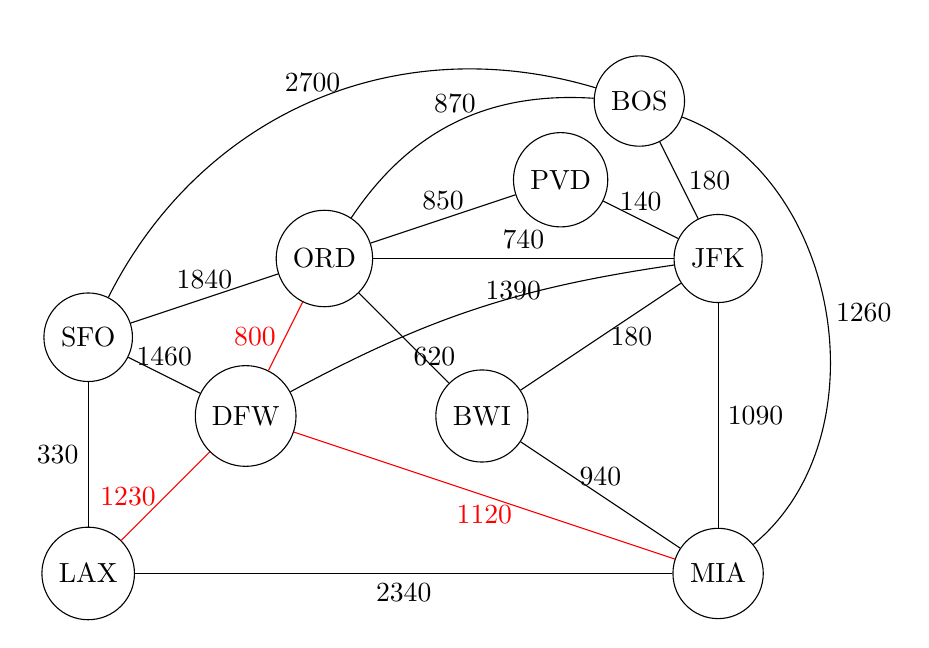
\begin{tikzpicture}[>=stealth]
    \node[ell] (sfo) at (1,8) {SFO};
    \node[ell] (lax) at (1,5) {LAX};
    \node[ell] (dfw) at (3,7) {DFW};
    \node[ell] (ord) at (4,9) {ORD};
    \node[ell] (bos) at (8,11) {BOS};
    \node[ell] (pvd) at (7,10) {PVD};
    \node[ell] (jfk) at (9,9) {JFK};
    \node[ell] (bwi) at (6,7) {BWI};
    \node[ell] (mia) at (9,5) {MIA};

    \draw [] (sfo) to []node[left]{330} (lax);
    \draw [] (sfo) to [bend left=40]node[above]{2700} (bos);
    \draw [] (sfo) to []node[above]{1840} (ord);
    \draw [] (sfo) to []node[above]{1460} (dfw);
    \draw [red] (lax) to []node[left]{1230} (dfw);
    \draw [] (lax) to []node[below]{2340} (mia);
    \draw [red] (dfw) to []node[left]{800} (ord);
    \draw [] (dfw) to [bend left=10]node[above right]{1390} (jfk);
    \draw [red] (dfw) to []node[below]{1120} (mia);
    \draw [] (ord) to []node[below right]{620} (bwi);
    \draw [] (ord) to []node[above]{740} (jfk);
    \draw [] (ord) to []node[above]{850} (pvd);
    \draw [] (ord) to [bend left]node[above]{870} (bos);
    \draw [] (pvd) to []node[above]{140} (jfk);
    \draw [] (bos) to []node[right]{180} (jfk);
    \draw [] (bos) to [bend left=60]node[right]{1260} (mia);
    \draw [] (jfk) to []node[right]{180} (bwi);
    \draw [] (jfk) to []node[right]{1090} (mia);
    \draw [] (mia) to []node[above]{940} (bwi);
\end{tikzpicture}
\begin{tabular}[b]{|c c c|} 
    \hline
    vertex $v$ & $v.d$ & $v.\pi$ \\
    \hline
    DFW & 0 & nil\\
    SFO & $\infty$ & nil \\
    LAX & 1230 & DFW \\
    ORD & 800 & DFW \\
    BOS & $\infty$ & nil \\
    PVD & $\infty$ & nil \\
    JFK & $\infty$ & nil \\
    BWI & $\infty$ & nil \\
    MIA & 1120 & DFW \\
    \hline
\end{tabular}
\\
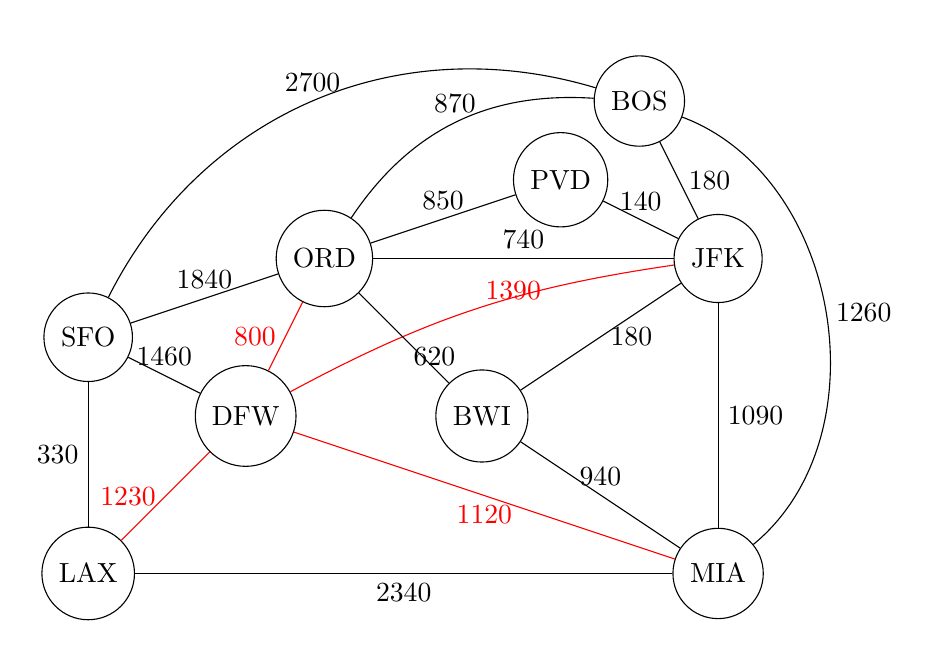
\begin{tikzpicture}[>=stealth]
    \node[ell] (sfo) at (1,8) {SFO};
    \node[ell] (lax) at (1,5) {LAX};
    \node[ell] (dfw) at (3,7) {DFW};
    \node[ell] (ord) at (4,9) {ORD};
    \node[ell] (bos) at (8,11) {BOS};
    \node[ell] (pvd) at (7,10) {PVD};
    \node[ell] (jfk) at (9,9) {JFK};
    \node[ell] (bwi) at (6,7) {BWI};
    \node[ell] (mia) at (9,5) {MIA};

    \draw [] (sfo) to []node[left]{330} (lax);
    \draw [] (sfo) to [bend left=40]node[above]{2700} (bos);
    \draw [] (sfo) to []node[above]{1840} (ord);
    \draw [] (sfo) to []node[above]{1460} (dfw);
    \draw [red] (lax) to []node[left]{1230} (dfw);
    \draw [] (lax) to []node[below]{2340} (mia);
    \draw [red] (dfw) to []node[left]{800} (ord);
    \draw [red] (dfw) to [bend left=10]node[above right]{1390} (jfk);
    \draw [red] (dfw) to []node[below]{1120} (mia);
    \draw [] (ord) to []node[below right]{620} (bwi);
    \draw [] (ord) to []node[above]{740} (jfk);
    \draw [] (ord) to []node[above]{850} (pvd);
    \draw [] (ord) to [bend left]node[above]{870} (bos);
    \draw [] (pvd) to []node[above]{140} (jfk);
    \draw [] (bos) to []node[right]{180} (jfk);
    \draw [] (bos) to [bend left=60]node[right]{1260} (mia);
    \draw [] (jfk) to []node[right]{180} (bwi);
    \draw [] (jfk) to []node[right]{1090} (mia);
    \draw [] (mia) to []node[above]{940} (bwi);
\end{tikzpicture}
\begin{tabular}[b]{|c c c|} 
    \hline
    vertex $v$ & $v.d$ & $v.\pi$ \\
    \hline
    DFW & 0 & nil\\
    SFO & $\infty$ & nil \\
    LAX & 1230 & DFW \\
    ORD & 800 & DFW \\
    BOS & $\infty$ & nil \\
    PVD & $\infty$ & nil \\
    JFK & 1390 & DFW \\
    BWI & $\infty$ & nil \\
    MIA & 1120 & DFW \\
    \hline
\end{tabular}
\\
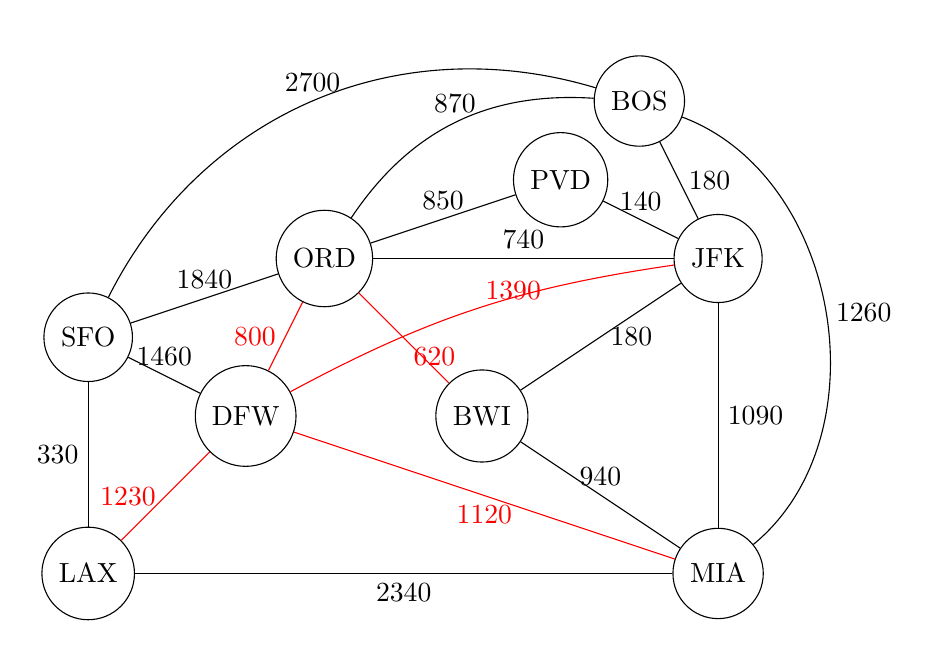
\begin{tikzpicture}[>=stealth]
    \node[ell] (sfo) at (1,8) {SFO};
    \node[ell] (lax) at (1,5) {LAX};
    \node[ell] (dfw) at (3,7) {DFW};
    \node[ell] (ord) at (4,9) {ORD};
    \node[ell] (bos) at (8,11) {BOS};
    \node[ell] (pvd) at (7,10) {PVD};
    \node[ell] (jfk) at (9,9) {JFK};
    \node[ell] (bwi) at (6,7) {BWI};
    \node[ell] (mia) at (9,5) {MIA};

    \draw [] (sfo) to []node[left]{330} (lax);
    \draw [] (sfo) to [bend left=40]node[above]{2700} (bos);
    \draw [] (sfo) to []node[above]{1840} (ord);
    \draw [] (sfo) to []node[above]{1460} (dfw);
    \draw [red] (lax) to []node[left]{1230} (dfw);
    \draw [] (lax) to []node[below]{2340} (mia);
    \draw [red] (dfw) to []node[left]{800} (ord);
    \draw [red] (dfw) to [bend left=10]node[above right]{1390} (jfk);
    \draw [red] (dfw) to []node[below]{1120} (mia);
    \draw [red] (ord) to [below right]node[]{620} (bwi);
    \draw [] (ord) to []node[above]{740} (jfk);
    \draw [] (ord) to []node[above]{850} (pvd);
    \draw [] (ord) to [bend left]node[above]{870} (bos);
    \draw [] (pvd) to []node[above]{140} (jfk);
    \draw [] (bos) to []node[right]{180} (jfk);
    \draw [] (bos) to [bend left=60]node[right]{1260} (mia);
    \draw [] (jfk) to []node[right]{180} (bwi);
    \draw [] (jfk) to []node[right]{1090} (mia);
    \draw [] (mia) to []node[above]{940} (bwi);
\end{tikzpicture}
\begin{tabular}[b]{|c c c|} 
    \hline
    vertex $v$ & $v.d$ & $v.\pi$ \\
    \hline
    DFW & 0 & nil\\
    SFO & $\infty$ & nil \\
    LAX & 1230 & DFW \\
    ORD & 800 & DFW \\
    BOS & $\infty$ & nil \\
    PVD & $\infty$ & nil \\
    JFK & 1390 & DFW \\
    BWI & 1420 & ORD \\
    MIA & 1120 & DFW \\
    \hline
\end{tabular}
\\
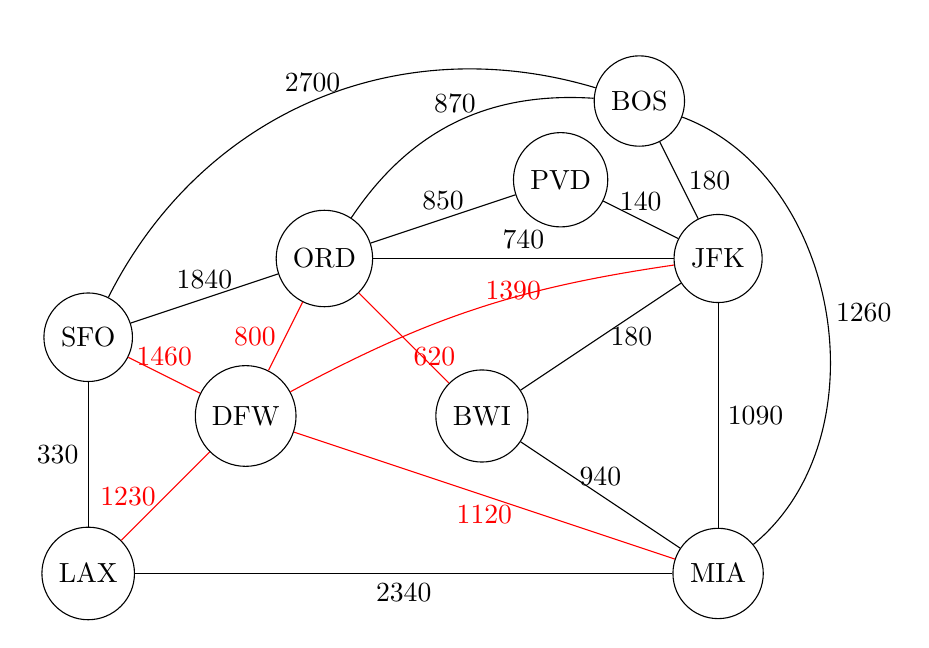
\begin{tikzpicture}[>=stealth]
    \node[ell] (sfo) at (1,8) {SFO};
    \node[ell] (lax) at (1,5) {LAX};
    \node[ell] (dfw) at (3,7) {DFW};
    \node[ell] (ord) at (4,9) {ORD};
    \node[ell] (bos) at (8,11) {BOS};
    \node[ell] (pvd) at (7,10) {PVD};
    \node[ell] (jfk) at (9,9) {JFK};
    \node[ell] (bwi) at (6,7) {BWI};
    \node[ell] (mia) at (9,5) {MIA};

    \draw [] (sfo) to []node[left]{330} (lax);
    \draw [] (sfo) to [bend left=40]node[above]{2700} (bos);
    \draw [] (sfo) to []node[above]{1840} (ord);
    \draw [red] (sfo) to []node[above]{1460} (dfw);
    \draw [red] (lax) to []node[left]{1230} (dfw);
    \draw [] (lax) to []node[below]{2340} (mia);
    \draw [red] (dfw) to []node[left]{800} (ord);
    \draw [red] (dfw) to [bend left=10]node[above right]{1390} (jfk);
    \draw [red] (dfw) to []node[below]{1120} (mia);
    \draw [red] (ord) to [below right]node[]{620} (bwi);
    \draw [] (ord) to []node[above]{740} (jfk);
    \draw [] (ord) to []node[above]{850} (pvd);
    \draw [] (ord) to [bend left]node[above]{870} (bos);
    \draw [] (pvd) to []node[above]{140} (jfk);
    \draw [] (bos) to []node[right]{180} (jfk);
    \draw [] (bos) to [bend left=60]node[right]{1260} (mia);
    \draw [] (jfk) to []node[right]{180} (bwi);
    \draw [] (jfk) to []node[right]{1090} (mia);
    \draw [] (mia) to []node[above]{940} (bwi);
\end{tikzpicture}
\begin{tabular}[b]{|c c c|} 
    \hline
    vertex $v$ & $v.d$ & $v.\pi$ \\
    \hline
    DFW & 0 & nil\\
    SFO & 1460 & DFW \\
    LAX & 1230 & DFW \\
    ORD & 800 & DFW \\
    BOS & $\infty$ & nil \\
    PVD & $\infty$ & nil \\
    JFK & 1390 & DFW \\
    BWI & 1420 & ORD \\
    MIA & 1120 & DFW \\
    \hline
\end{tabular}
\\
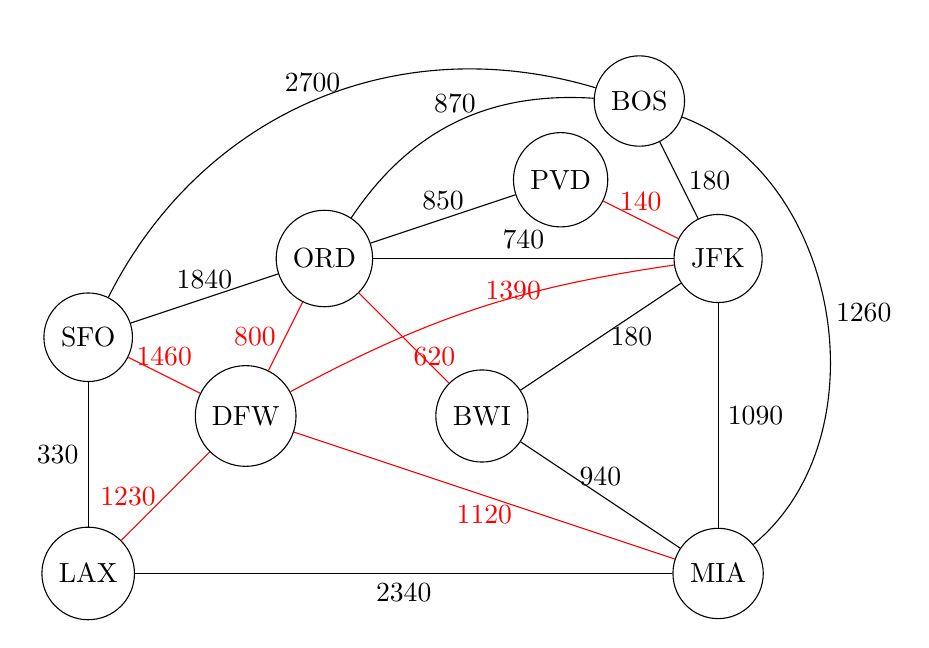
\begin{tikzpicture}[>=stealth]
    \node[ell] (sfo) at (1,8) {SFO};
    \node[ell] (lax) at (1,5) {LAX};
    \node[ell] (dfw) at (3,7) {DFW};
    \node[ell] (ord) at (4,9) {ORD};
    \node[ell] (bos) at (8,11) {BOS};
    \node[ell] (pvd) at (7,10) {PVD};
    \node[ell] (jfk) at (9,9) {JFK};
    \node[ell] (bwi) at (6,7) {BWI};
    \node[ell] (mia) at (9,5) {MIA};

    \draw [] (sfo) to []node[left]{330} (lax);
    \draw [] (sfo) to [bend left=40]node[above]{2700} (bos);
    \draw [] (sfo) to []node[above]{1840} (ord);
    \draw [red] (sfo) to []node[above]{1460} (dfw);
    \draw [red] (lax) to []node[left]{1230} (dfw);
    \draw [] (lax) to []node[below]{2340} (mia);
    \draw [red] (dfw) to []node[left]{800} (ord);
    \draw [red] (dfw) to [bend left=10]node[above right]{1390} (jfk);
    \draw [red] (dfw) to []node[below]{1120} (mia);
    \draw [red] (ord) to [below right]node[]{620} (bwi);
    \draw [] (ord) to []node[above]{740} (jfk);
    \draw [] (ord) to []node[above]{850} (pvd);
    \draw [] (ord) to [bend left]node[above]{870} (bos);
    \draw [red] (pvd) to []node[above]{140} (jfk);
    \draw [] (bos) to []node[right]{180} (jfk);
    \draw [] (bos) to [bend left=60]node[right]{1260} (mia);
    \draw [] (jfk) to []node[right]{180} (bwi);
    \draw [] (jfk) to []node[right]{1090} (mia);
    \draw [] (mia) to []node[above]{940} (bwi);
\end{tikzpicture}
\begin{tabular}[b]{|c c c|} 
    \hline
    vertex $v$ & $v.d$ & $v.\pi$ \\
    \hline
    DFW & 0 & nil\\
    SFO & 1460 & DFW \\
    LAX & 1230 & DFW \\
    ORD & 800 & DFW \\
    BOS & $\infty$ & nil \\
    PVD & 1530 & JFK \\
    JFK & 1390 & DFW \\
    BWI & 1420 & ORD \\
    MIA & 1120 & DFW \\
    \hline
\end{tabular}
\\
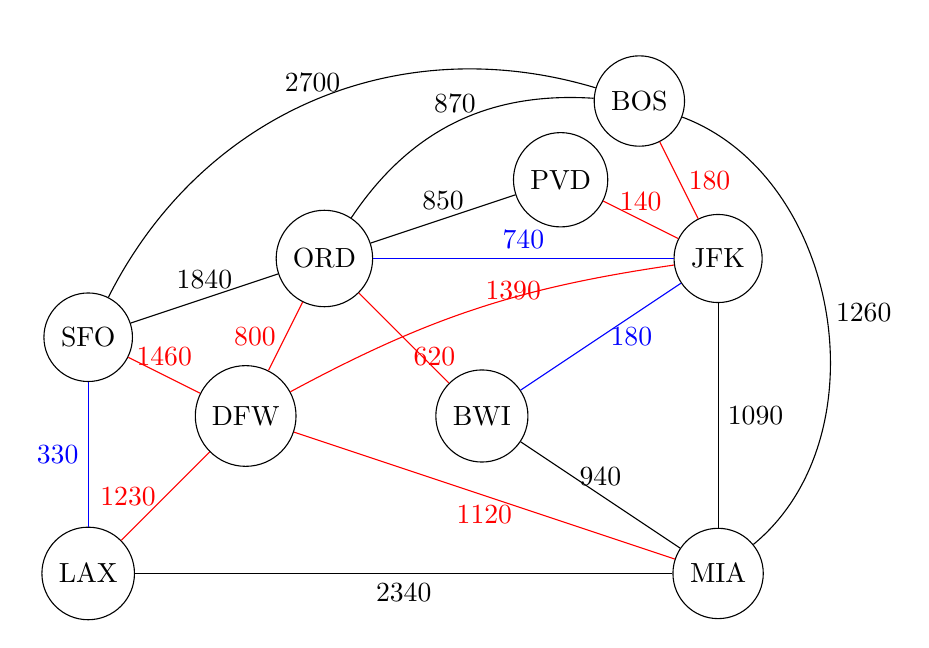
\begin{tikzpicture}[>=stealth]
    \node[ell] (sfo) at (1,8) {SFO};
    \node[ell] (lax) at (1,5) {LAX};
    \node[ell] (dfw) at (3,7) {DFW};
    \node[ell] (ord) at (4,9) {ORD};
    \node[ell] (bos) at (8,11) {BOS};
    \node[ell] (pvd) at (7,10) {PVD};
    \node[ell] (jfk) at (9,9) {JFK};
    \node[ell] (bwi) at (6,7) {BWI};
    \node[ell] (mia) at (9,5) {MIA};

    \draw [blue] (sfo) to []node[left]{330} (lax);
    \draw [] (sfo) to [bend left=40]node[above]{2700} (bos);
    \draw [] (sfo) to []node[above]{1840} (ord);
    \draw [red] (sfo) to []node[above]{1460} (dfw);
    \draw [red] (lax) to []node[left]{1230} (dfw);
    \draw [] (lax) to []node[below]{2340} (mia);
    \draw [red] (dfw) to []node[left]{800} (ord);
    \draw [red] (dfw) to [bend left=10]node[above right]{1390} (jfk);
    \draw [red] (dfw) to []node[below]{1120} (mia);
    \draw [red] (ord) to [below right]node[]{620} (bwi);
    \draw [blue] (ord) to []node[above]{740} (jfk);
    \draw [] (ord) to []node[above]{850} (pvd);
    \draw [] (ord) to [bend left]node[above]{870} (bos);
    \draw [red] (pvd) to []node[above]{140} (jfk);
    \draw [red] (bos) to []node[right]{180} (jfk);
    \draw [] (bos) to [bend left=60]node[right]{1260} (mia);
    \draw [blue] (jfk) to []node[right]{180} (bwi);
    \draw [] (jfk) to []node[right]{1090} (mia);
    \draw [] (mia) to []node[above]{940} (bwi);
\end{tikzpicture}
\begin{tabular}[b]{|c c c|} 
    \hline
    vertex $v$ & $v.d$ & $v.\pi$ \\
    \hline
    DFW & 0 & nil\\
    SFO & 1460 & DFW \\
    LAX & 1230 & DFW \\
    ORD & 800 & DFW \\
    BOS & 1570 & JFK \\
    PVD & 1530 & JFK \\
    JFK & 1390 & DFW \\
    BWI & 1420 & ORD \\
    MIA & 1120 & DFW \\
    \hline
\end{tabular}
\end{problem}
% --------------------------------------------------------------
%     You don't have to mess with anything below this line.
% --------------------------------------------------------------
 
\end{document}